% ai-based-phishing-detection-dissertation/report/main.tex

\documentclass[
  pdftex,
  10pt,
  a4paper,
  oneside
]{article}

% Packages
% ai-phishing-detection-dissertation/report/preamble/packages.tex

\usepackage{amsmath}
\numberwithin{equation}{section}
\usepackage{algorithm}
\usepackage{algorithmic}
\usepackage{fancyhdr}
\usepackage{graphicx}
\graphicspath{ {images/} }
\usepackage{setspace}
\usepackage[]{fncychap}
\usepackage[hyphens]{url}
\usepackage{xcolor}
\usepackage{tabularx}
\usepackage{appendix}
\usepackage[hidelinks]{hyperref}
\usepackage{pdfpages}
\usepackage[round]{natbib}
\usepackage[a4paper,margin=1in]{geometry}
\usepackage{longtable}
\usepackage{caption}
\usepackage{pdflscape}
\usepackage{lscape}
\usepackage[normalem]{ulem}
\usepackage{ffcode}
\usepackage{amsfonts}
\usepackage{amssymb}
\usepackage{float}
\usepackage{ffcode}

% Fancy header/footer
% ai-phishing-detection-dissertation/report/preamble/fancy-header-footer.tex

\fancyhf{}
\pagestyle{fancy}
\renewcommand{\headrulewidth}{0.2pt}
\fancyfoot[C]{\thepage}


\begin{document}

  % Preamble
   % Remove headers/footers for the title page
\thispagestyle{empty}

% Double spacing for the title page
\begin{spacing}{2}
    \begin{center}

        % University Crest
        
\includegraphics[scale=0.45]{preamble/warwick-crest.pdf}
        \vspace{10mm}

        % Dissertation Title
        \textbf{\LARGE AI Phishing Detection with Explainable AI}
        \vspace{20mm}

        % Student ID
        {\large \textbf{Student ID: 2242090}}
        \vspace{20mm}

        % Supervisor and Department
        {\large Supervisor: Sarah Aktaa}\\
        \textbf{\large Department of Warwick Manufacturing Group (WMG)}\\
        {\large University of Warwick}\\
        {\large Academic Year: 2024-2025}

    \end{center}
\end{spacing}

% Start Roman numbering for front matter
\pagenumbering{arabic}

  \newpage
  % ai-phishing-detection-dissertation/report/preamble/abstract.tex

\section*{Abstract}
\addcontentsline{toc}{section}{Abstract}

Phishing attacks are known to be a big challenge in cybersecurity. Whilst Artificial Intelligence (AI) can help in detecting and preventing such attacks, most models are "black-boxed", and this limits user trust. This study therefore researches the practical development of an AI-powered phishing detection by implementing and evaluating two distinct models: a Random Forest classifier with TF-IDF features and a fine-tuned DistilBERT transformer. Explainable AI (XAI) techniques, such as SHAP for Random Forest and LIME for DistilBERT, were integrated to enhance model transparency. Both models achieved high accuracies of over 98\% on an internal test set comprised of Enron and CEAS 08 corpora. Evaluations on independent, extenal datasets (SpamAssassin, Nigerian Fraud, Nazario) revealed generalisation challenges. Although there was a high precision for phishing instances, there was equally as low recall. The XAI methods integrated provide both global and local explanations, showing how features and words contributed to the model's final outcome.\newline

\large
\noindent This project aligns with the following CyBok Skills: \textbf{Malware \& Attack Technologies}, \textbf{Human Factors}, \textbf{Adversarial Behaviours}.
  \newpage
  \section*{Acknowledgements}
\addcontentsline{toc}{section}{Acknowledgements}


  \newpage
  % ai-phishing-detection-dissertation/report/preamble/abbreviations.tex

\section*{Abbreviations}
\addcontentsline{toc}{section}{Abbreviations}

\large
Artificial Intelligence \hfill AI\\
Anti-Phishing Working Group \hfill APWG\\
Challenge Lab Evaluation Corpus \hfill CEAS\\
Deep Learning \hfill HL\\
Explainable Boosting Machines \hfill EBM\\
General Data Protection Regulation \hfill GDPR\\
Global Digital Population \hfill GDP\\
Gated Recurrent Unit Long Short-Term Memory \hfill GRU-LSTM\\
K-Nearest Neighbours \hfill KNN\\
Large Language Model \hfill LLM\\
Local Interpretable Model-agnostic Explanations \hfill LIME\\
Machine Learning \hfill ML\\
Natural Language Processing \hfill NLP \\
SHapley Additive exPlanations \hfill SHAP\\
Simple Vector Machine \hfill SVM\\
Uniform Resource Locator \hfill URL\\
Voice over Internet Protocol \hfill VoIP\\
eXplainable Artificial Intelligence \hfill XAI\\
eXplainable Artificial Intelligence with\newline Aquila Optimization Algorithm in Web Phishing Classification \hfill XAIAOA-WPC\\
eXplainable Artificial Intelligence Ensemble-based Filter Feature Selection \hfill XAI-EFFS\\
University of New Brunswick \hfill UNB\\


  \newpage
  % ai-phishing-detection-dissertation/report/preamble/contents.tex

\setcounter{tocdepth}{2}
\tableofcontents


  \newpage
  % % ai-phishing-detection-dissertation/report/preamble/lists.tex

\listoffigures
\addcontentsline{toc}{section}{List of Figures}
\numberwithin{figure}{section}

\listoftables
\addcontentsline{toc}{section}{List of Tables}
\numberwithin{table}{section}

\listofalgorithms
\addcontentsline{toc}{section}{List of Algorithms}
\numberwithin{algorithm}{section}


  % \newpage

  % Page stylings
  \pagenumbering{arabic}

\lfoot{\centering \thepage}

  % ai-phishing-detection-dissertation/report/preamble/landscape-style.tex

\fancypagestyle{mylandscape}{
  \fancyhf{} % Clear header and footer
  \fancyfoot[R]{\rotatebox{90}{\centering \thepage}} % Rotate the page number
  \renewcommand{\headrulewidth}{0pt} % No header rule
  \renewcommand{\footrulewidth}{0pt} % No footer rule
}



  \newpage

  % Sections

  % 1: Introduction
  \section{Introduction}\label{sec:1-introduction}

  % 1.1: Background
  \subsection*{Background}

It is deemed that phishing attacks are one of the most common forms of cyber crimes today, with its targets ranging from individuals to large-scale organisations, with the aim of obtaining sensitive information including personal identification, credentials, and financial data. Acording to the DataBreach Report by \cite{verizon2023}, it was investigated that social engineering was responsible for over 50\% of all breaches -- a significant point to consider for cybersecurity. The attacks mainly use complex social engineering techniques such as deceptive content, malicious URLs posing as legitimate, and impersonation, all in an attempt to bypass traditional security systems \citep{marett2009effectiveness}. \newline

\noindent Therefore, Artificial intelligence (AI) and machine learning (ML) can serve as effective tools in detecting phishing attempts. Models can be trained on huge datasets on features like suspicious email headers, text anomalies, and malicious links, which humans have a high probability of missing (\cite{chandrasekaran2006phoney}; \cite{jain2022survey}). However, it is important to note that most traditional AI-phishing detection systems function as a "black-box" model, and they don't offer much transparency into their decision-making processes. Since there is little to no interpretability, it not only reduces trust on the user's side, but the risk that these systems carry inhibit it from being implemented in high-stakes environments such as financial institutions and governmental agencies \citep{ribeiro2016model}. \newline

\noindent Explainable AI (XAI) solve this challenge by attempting to make AI systems more understandable and transparent. Techniques like SHAP (SHapley Additive Explanations) and LIME (Local Interpretable Model-agnostic Explanations) can give insights into the prediction process models undergo (\cite{lundberg2017unified}; \cite{ribeiro2016model}). Especially for phishing detection, XAI can very much empower a user's confidence in understanding why an email is flagged, due to either language cues, suspicious links, or email metadata. \newline

\noindent However despite advances in AI and XAI, there still remain gaps into integrating explainability into phishing detection models. Many existing approaches have a prioritisation on accuracy, without much thought for comprehensability \citep{hernandes2021phishing}. This means its difficult to strike a balance between performance and transparency. This project therefore addresses to seek this gap, by developing an XAI-enhanced phishing detection system that achieves a high accuracy whilst providing actionable explanations behind its predictions.


  % 1.2: Objectives
  % ai-phishing-detection-dissertation/report/sections/1-introduction/objectives.tex

\subsection{Objectives}

\begin{enumerate}
  \item \uline{\textbf{OBJECTIVE 1}}: "\textit{Conduct a comprehensive review of existing AI phishing detection models}.\label{objective-1}"
  \begin{itemize}
    \item Review existing AI phishing detection systems.
    \item Identify research gaps to address in relation to interpretability in phishing detection.
    \item Explore XAI techniques, like SHAP and LIME, and their applicability for phishing detection
    \end{itemize}
  \item \uline{\textbf{OBJECTIVE 2}}: "\textit{Identify and implement suitable XAI techniques (e.g., SHAP, LIME)}.\label{objective-2}"
  \begin{itemize}
    \item Develop upon a traditional model already being used for phishing detection, e.g. Random Forest or Transformer-based models.
    \item Integrate XAI techniques into these models that can explain the model predictions.
    \item Achieve a competitive accuracy that is either on par or better than existing AI-based phishing detection models.
  \end{itemize}
\item \uline{\textbf{OBJECTIVE 3}}: "\textit{Evaluate the system's performance in terms of accuracy and interpretability}.\label{objective-3}"
  \begin{itemize}
    \item Assess the system on performance metrics such as precision, accuracy, and recall.
    \item Analyse how useful explanations are using standard interpretability metrics.
  \end{itemize}
\item \uline{\textbf{OBJECTIVE 4}}: "\textit{Compare the usability of the XAI phishing detection model with traditional black-boxed models}.\label{objective-4}"
  \begin{itemize}
    \item Conduct small-scale user studies or surveys to determine how effective XAI influences usability and trust -- compared to black-boxed phishing detection models.
    \item Discuss whether or not its worth compromising on accuracy to achieve trust and usability.
  \end{itemize}
\end{enumerate}


  % 1.3: Research questions
  \subsection*{Research questions}

\begin{enumerate}
    \item \textbf{Primary research question:}
        \begin{itemize}
            \item \textit{How can Explainable AI (XAI) improve the usability and trustworthiness of AI-based phishing detection systems without compromising on accuracy?}
        \end{itemize}
    \item \textbf{Sub-questions:}
        \begin{itemize}
            \item What are the current limitations of AI phishing detection models in terms of their usability and interpretability?
            \item How do the interpretability features affect a user's trust building and decision-making processes?
            \item How can XAI techniques, i.e. SHAP and LIME, be integrated efficiently on top of existing AI phishing detection models?
            \item What trade-offs, if any, arise between the performance and interpretability of the AI phishing detection model?
        \end{itemize}
\end{enumerate}


  % 1.4: Structure
  \subsection*{Paper structure}

The paper is structured as follows: \hyperref[sec:2-literature-review]{Section 2} is the result of a comprehensive literature review into the space of AI-based phishing detection, which neatly progresses onto the relevance of XAI in this field. \hyperref[sec:3-research-methodology]{Section 3} discusses the research methodology, and the practical implementation of the XAI-enhanced phishing detection model.



  \newpage

  % 2: Literature review
  \section{Literature review}\label{sec:2-literature-review}
  % ai-phishing-detection-dissertation/report/sections/3-research-methodology/model-development/introduction.tex



  % 2.1: AI-based phishing detection models
  \subsection{AI-based phishing detection models}
  % ai-phishing-detection-dissertation/report/sections/2-literature-review/ai-based-phishing-detection-models/limitations-of-traditional-phishing-detection.tex

\subsubsection*{Limitations of traditional phishing detection}

  % ai-phishing-detection-dissertation/report/sections/2-literature-review/ai-based-phishing-detection-models/ml-models-for-phishing-detection.tex

\subsubsection*{ML models for phishing detection}
AI-driven phishing detection systems have therefore emerged as a potential alternative to traditional machine learning, as stated by \cite{do2022deep}, especially in this context. In particular, they mention how deep learning models, can be applied to detect phishing content in various areas such as websites, emails, mobile devices, VoIP, and so on, achieving competitive accuracies when compared to traditional ML models. \cite{tang2021survey} supports this, by also mentioning how machine learning algorithms, such as neural networks, linear regression, logistic regression, decision trees, SVM, KNN, and random forest, have a high suitability when it comes to a supervised classification tasks like phishing detection. Specifically, models such as random forest have boasted a high performance in a study conducted by \cite{gupta2021novel}, achieving an accuracy of 99.57\%. Research by \citep{kapoor2024comparative} also advocated for the outstanding performance of random forest, especially in its ability to maintain a classification balance, minimising the risk of false positives and negatives.Other models such as KNN and random forest have achieved similar accuracies, 97.2\%, as seen in the study by \cite{zamir2020phishing}. But all studies note on agree on using a hybrid approach of several models in combination can lead to better detection performance, with an example of using multiple classifiers in \cite{alsariera2020ai} or using a hybrid feature selection process as showcased by \cite{hamid2013using}.

  % ai-phishing-detection-dissertation/report/sections/2-literature-review/ai-based-phishing-detection-models/dl-and-transformer-based-models.tex

\subsubsection*{DL and transformer-based models}
Additionally, transformer based models have been shown to perform equally as well, with a study by \cite{do2024integrated} presenting a model with a 99.71\% detection accuracy. Another study by \cite{shirazi2022towards} agrees with this notion, particularly highlighting the significance of pre-trained transformer models showing substantial performance compared to other current approaches, despite their lower accuracy scores. Their advantage lies in the fact that they do not require pre-processing as certain features -- making them highly adaptable for feature-driven detection. Not only that, but the study claims that transformer-based models are more practical for organisations, since they are faster and require less training time \citep{shirazi2022towards}.

  % ai-phishing-detection-dissertation/report/sections/2-literature-review/ai-based-phishing-detection-models/practical-benefits-and-future-potential.tex

\subsubsection*{Practical benefits and future potential}


  % 2.2: Challenges in AI-based phishing detection
  \subsection{Challenges in AI-based phishing detection}
  % ai-phishing-detection-dissertation/report/sections/2-literature-review/challenges-in-ai-based-phishing-detection/dataset-and-model-performance-issues.tex

\subsubsection*{Dataset and model performance issues}
Some simpler models, such as decision trees and random forest, are seen to suffer from a case of overfitting due to the imbalance of datasets and high dimensional data, demonstrated in a study by \cite{harikrishnan2018machine}. A large majority of the reasons as to the performance drop-off is due to dataset limitations like lack of specific features or dataset size, as observed by \cite{ahmad2024across}. They mainly noted how datasets struggled to perform well due to a lack of quality and diverse data. Training times were a significant challenge, not just from dataset size, but the inherent nature of deep learning models (consisting of many layers), that might limit their applicability in real-time situations, as discovered by \cite{kapoor2024comparative}, which is also agreed upon by \cite{atlam2022business}.

  % ai-phishing-detection-dissertation/report/sections/2-literature-review/challenges-in-ai-based-phishing-detection/adversarial-evolution-and-scalability.tex

\subsubsection*{Adversarial evolution and scalability}
In \cite{kapoor2024comparative}'s research, they also comment on the constant evolution of sophisticated tactics introduced by attackers, such a deep fakes, new social engineering tactics, and context-aware attacks -- all with the goal of exploiting human technology. They mention that it is important to factor in an "arms race" between AI models being trained on new data and attackers coming up with new intrusion methods. Traditional models, apart from overfitting, suffer from their sensitivity to parameter turning such as SVM \citep{andriu2023adaptive}. Furthermore, it is a challenge to scale these models given the ever-growing needs of an organisation, as the system must be able to both maintain its performance and optimal detection to deal with increasing workloads, with a lack of real-time implementations and studies, observed by \cite{atlam2022business}.

  % ai-phishing-detection-dissertation/report/sections/2-literature-review/challenges-in-ai-based-phishing-detection/privacy-and-error-trade-offs.tex

\subsubsection*{Privacy and error trade-offs}
GDPR comes into play here as these systems use user information from email content and metadata, so they need to be ensure compliance and have the appropriate privacy mechanisms implemented. Models are also likely to fall victim of flagging false positives and negatives, and this is a vital aspect in keeping them from being deployed in a real-time setting, emphasised by \cite{vishwanath2011people}. False positives can logically cause disruption and inconvenience for businesses and users respectively, where as false negatives are phishing emails that may bypass filters introducing a vulnerability. It is vital for models to prioritise a balance between these two categories of errors for a practical phishing detection system.

  % ai-phishing-detection-dissertation/report/sections/2-literature-review/challenges-in-ai-based-phishing-detection/interpretability-and-xai-challenges.tex

\subsubsection*{Interpretability and XAI challenges}
Another key area is interpretability challenges mentioned by \cite{atlam2022business}, as they state how most AI models are "black-boxed" from users. Only input and output data can be seen, but the process in between are often obscured. The authors drive forward the point of introducing XAI to allow these models to be interpretable, lading to more dependence and instill a sense of confidence in their decisions. There are other studies, such as by \cite{al2024novel}, that note the challenges associated with interpreting feature importance with non-linear models. But the novelty of XAI in general poses several questions which are addressed in the study by \cite{yakandawala2023review}, where several XAI challenges are listed. The most notable being able to strike the perfect balance between explainability and performance. A model that is non-explainable can receive "public backlash" due to AI errors and biases, lessening trust in their decision making processes. This especially affects deep learning models which face a lot more interpretability issues than other models due to their complexity. A study to complement this, by \cite{reddy2023explainable}, that suggest several more issues concerning interpretability, such a lack of a universal standard or rigid framework in which to develop and evaluate these XAI techniques. The authors claim that is it important to take human factors into account, and it would prove to be effective to understand how users would interact with such explanations.

  % ai-phishing-detection-dissertation/report/sections/2-literature-review/challenges-in-ai-based-phishing-detection/ethical-and-human-factor-concerns.tex

\subsubsection*{Ethical and human-factor concerns}


  % 2.3: XAI in the context of phishing detection
  \subsection{XAI in the context of phishing detection}
  % ai-phishing-detection-dissertation/report/sections/2-literature-review/xai-in-the-context-of-phishing-detection/introduction-to-xai-and-its-importance.tex

\subsubsection*{Introduction to XAI and its importance}
There are many studies that put forward the solution of XAI to address interpretability and transparency issues \citep{roshan2022using} associated with systems that employ ML techniques. The goal of XAI here is to serve as a means to understand and inspire confidence in an AI's decision making processes \citep{khanom2025pd_ebm}, from the input all the way through to the output (\citeauthor{jawale2020jeevn}, \citeyear{jawale2020jeevn}; \citeauthor{sanchez2022phishing}, \citeyear{sanchez2022phishing}), with use cases for analysts being able to differentiate between false positives and negatives \citep{van2024applicability}. In particular, there are several existing studies into how XAI plays a role in the context of phishing detection, with a study by \cite{alzahrani2024explainable} proving that both high accuracies (97\%) and reasonable explainability features can be achieved. The importance of such explainable systems is stressed by \cite{shendkar2024enhancing} and further literature comments on how there's been a recent interest for outcome explanations for textual and document based classification tasks (\citeauthor{martens2014explaining}, \citeyear{martens2014explaining}; \citeauthor{lei2016rationalizing}, \citeyear{lei2016rationalizing}).

  % ai-phishing-detection-dissertation/report/sections/2-literature-review/xai-in-the-context-of-phishing-detection/user-centric-challenges-and-psychological-factors.tex

\subsubsection*{User-centric challenges and psychological factors}

  % ai-phishing-detection-dissertation/report/sections/2-literature-review/xai-in-the-context-of-phishing-detection/xai-techniques-and-methodologies.tex

\subsubsection*{XAI techniques and methodologies}
There are many ways this can be achieved, and this moves the literature review to specific XAI techniques that can be utilised and practically implemented into AI-powered systems, such as SHAP and LIME as a way to offer insights \citep{shendkar2024enhancing} by providing both global and localised explanations, respectively \citep{palaniappan2020malicious}. There is also an additional higher level explainability technique, EBM, refered to by \cite{hernandes2021phishing}, that is a complete white-boxed approach that aims to construct a predictive model that is already inherently explainable by design and does not require additional interpretability tools post processing \citep{greco2023explaining}. Comparing this with LIME, it builds an interpretation based upon existing black-boxed models' outcomes. Both these techniques provide local and global explanations and are model-agnostic, i.e. they can work with any model or classifier that's ML-based \citep{anderson2015polymorphic}. \cite{greco2023explaining} also dives deeper into the different between local and global explanations, adding onto previous understanding. The author mentiones that local explanations consist of a "feature importance vector" which is a quantifiable value that shows how much that specific feature contributed to the outcome. This is constrating to global explanations, as they require both the entire model and its processing mechanisms.

  % ai-phishing-detection-dissertation/report/sections/2-literature-review/xai-in-the-context-of-phishing-detection/practical-implementations-and-case-studies.tex

\subsubsection*{Practical implementations and case studies}
A contextual example of these techniques being implemented is the Phishpedia model presented in research by \cite{lin2021phishpedia}, where it takes URLs and returns an explanation to the user based on the legitimacy of its web domain. The important thing here to note is the attention to user feedback, in the form of dialog boxes as previously mentioned. The alert is very visually appealing and informative to the user, with an emphasis on why the URL is potentially malicious, making compairons of known URLs with proper web domains. Another interpretable approach by \cite{bravo2010bridging} is using a phishing email's metadata and content, showing whether each feature (if any), contributed to its final classification of phishing (or not phishing). A very recent study, \cite{lim2025explicate}, designed an XAI and LLM enhanced phishing detection system called EXPLICATE, utilising LIME, SHAP on a DeepSeek v3 base model with a very practical balance achieved between interpretability, accuracy, and efficiency. There are also specialised, innovative XAI approaches, such as XAIAOA-WPC talked about in research by \cite{alotaibi2025explainable} that boasts a high performance rate of 99.29\%, incorporating mainly LIME for its explainability. There are also systems which employ SHAP, such as the integrated intelligence defender framework, CyberDefender proposed by \cite{krishnaveni2024cyberdefender} that utilised a similar custom XAI solution, called XAI-EFFS, which is a filter feature selection that is ensemble-based. This specific solution takes existing hyper-parameters of a GRU-LSTM deep learning model that used optimisation tactics that are Bayesian-inspired. Feature importance analysis can also be supplemented by XAI, as explored by \cite{fajar2024enhancing}, who discovered that the combination of both RFE and XAI could correctly identify distinct dataset features that largely influenced the model's final decision. In this study, the XGBoost and CatBoost models maintined high accuracy and efficiency, with the former being more scalable and the latter being more robust.

  % ai-phishing-detection-dissertation/report/sections/2-literature-review/xai-in-the-context-of-phishing-detection/future-directions.tex

\subsubsection*{Future directions}
To conclude, it is safe to say that there are plenty of integrations of XAI with phishing detection models, often achieving competitive accuracies along with interpretability features. A range of XAI techniques are implemented, the most common being SHAP and LIME, with some uses of EBM. However, there lies some areas that need to be addressed as emphasised by most studies' future works.


  % 2.4: Research gaps
  \subsection{Research gaps}
  % ai-phishing-detection-dissertation/report/sections/3-research-methodology/model-development/introduction.tex


  % ai-phishing-detection-dissertation/report/sections/2-literature-review/research-gaps/research-gap-1.tex

\subsubsection*{Research gap 1: Interpretability vs. performance trade-offs in phishing detection systems}\label{research-gap-1}
Higher accuracy models, such as transformers and random forest, often lack many interpretability features. More explainable models like EBM may underperform (\citeauthor{do2024integrated}, \citeyear{do2024integrated}; \citeauthor{greco2023explaining}, \citeyear{greco2023explaining}). There are few studies that find the optimal balance between the two. Aligned with \hyperref[objective-2]{\uline{\textbf{Objective 2}}} and \hyperref[sub-research-q4]{\uline{\textbf{Sub Research Question 4}}}.

  % ai-phishing-detection-dissertation/report/sections/2-literature-review/research-gaps/research-gap-2.tex

\subsubsection*{Research gap 2: Lack of a user-centric XAI design}\label{research-gap-2}
Most of the existing XAI-powered systems focus on technical explanations of outputs, such as with SHAP/LIME. They fail to evaluate how users interact with them (\citeauthor{vo2024securing}, \citeyear{vo2024securing}; \citeauthor{anderson2015polymorphic}, \citeyear{anderson2015polymorphic}). Aligned with \hyperref[objective-4]{\uline{\textbf{Objective 4}}} and \hyperref[sub-research-q2]{\uline{\textbf{Sub Research Question 2}}}.

  \vspace{-0.5cm}
  % ai-phishing-detection-dissertation/report/sections/2-literature-review/research-gaps/research-gap-3.tex

\subsubsection*{Research gap 3: Absence of standardised XAI evaluation metrics}\label{research-gap-3}
There isn't a rigid framework nor a consensus on how to formally assess XAI's effectiveness for phishing detection (\citeauthor{reddy2023explainable}, \citeyear{reddy2023explainable}; \citeauthor{shendkar2024enhancing}, \citeyear{shendkar2024enhancing}). Aligned with \hyperref[objective-3]{\uline{\textbf{Objective 3}}}.


  % ai-phishing-detection-dissertation/report/sections/2-literature-review/research-gaps/research-gap-4.tex

\subsubsection*{Research gap 4: Limited real-world validation of XAI phishing detection systems}\label{research-gap-4}
Most studies test models in controlled environments and often ignore real-world limitations such as privacy (GDPR) compliance and scalability means (\citeauthor{kapoor2024comparative}, \citeyear{kapoor2024comparative}; \citeauthor{atlam2022business}, \citeyear{atlam2022business}). Aligned with \hyperref[sub-research-q1]{\uline{\textbf{Sub Research Question 1}}}.

  % ai-phishing-detection-dissertation/report/sections/2-literature-review/research-gaps/research-gap-5.tex

\subsubsection*{Research gap 5: Inadequate integration of XAI with high performing AI models}\label{research-gap-5}
Whilst its known that SHAP/LIME can be applied to traditional ML models, such as random forest and decision trees, their integration with more complex models like transformers or hybrid  architectures isn't substantially explored (\citeauthor{alzahrani2024explainable}, \citeyear{alzahrani2024explainable}; \citeauthor{lim2025explicate}, \citeyear{lim2025explicate}). Aligned with \hyperref[objective-1]{\uline{\textbf{Objective 1}}} and \hyperref[objective-2]{\uline{\textbf{Objective 2}}}.

  % ai-phishing-detection-dissertation/report/sections/2-literature-review/research-gaps/research-gap-6.tex

\subsubsection*{Research gap 6: Dynamic adaptability to evolving phishing tactics}\label{research-gap-6}
Studies have AI models trained on static dataset, and as a result, they fail with novel attack vectors, which includes deepfakes and context-aware attacks (\citeauthor{kapoor2024comparative}, \citeyear{kapoor2024comparative}; \citeauthor{atlam2022business}, \citeyear{atlam2022business}). There are few studies that take continous training into consideration, along with XAI to explain the adaptations models make. Aligned with \hyperref[objective-1]{\uline{\textbf{Objective 1}}} and \hyperref[sub-research-q1]{\uline{\textbf{Sub Research Question 1}}}.

  % ai-phishing-detection-dissertation/report/sections/2-literature-review/research-gaps/research-gap-7.tex

\subsubsection*{Research gap 7: Bias and fairness in XAI interpretability explanations}\label{research-gap-7}
Some studies show that XAI techniques can be influenced from biases in training data, for example flagging emails from specific domains as phishign by default \citep{hanif2021survey}. As of now, there are no studies that account for this bias for phishing-specific XAI outcomes. Aligned with \hyperref[objective-3]{\uline{\textbf{Objective 3}}}.

  % ai-phishing-detection-dissertation/report/sections/2-literature-review/research-gaps/research-gap-8.tex

\subsubsection*{Research gap 8: Computational overhead of XAI integration}\label{research-gap-8}
Studies which attempt real-time deployment are often limited by the computational costs of the inherent model as well as the additional XAI techniques, i.e. SHAP/LIME latency \citep{kapoor2024comparative}. There isn't much numerical analysis on efficiency and speed. Aligned with \hyperref[sub-research-q4]{\uline{\textbf{Sub Research Question 4}}}.

  % ai-phishing-detection-dissertation/report/sections/2-literature-review/research-gaps/research-gap-9.tex

\subsubsection*{Research gap 9: Interdisciplinary explanations for non-technical users}\label{research-gap-9}
XAI outputs from models that studies have developed often assume technical expertise of the user \citep{greco2023explaining}. There are no current frameworks that adapt XAI explanations to various user roles, such as from a SOC analyst to an end-user. Aligned with \hyperref[objective-4]{\uline{\textbf{Objective 4}}} and \hyperref[sub-research-q2]{\uline{\textbf{Sub Research Question 2}}}.


  % ai-phishing-detection-dissertation/report/sections/2-literature-review/research-gaps/research-gap-10.tex

\subsubsection*{Research gap 10: Privacy respecting XAI for compliance}\label{research-gap-10}
Since phishing detectors often process sensitive user information extracted from email metadata and content, models have to be privacy respecting. XAI explanations carry the risk of leaking sensitive user data \citep{atlam2022business}. GDPR-compliant XAI implementations are yet to be explored. Aligned with \hyperref[sub-research-q1]{\uline{\textbf{Sub Research Question 1}}}.


  % 2.5: Justification for this study
  \subsection{Justification for this study}
  % ai-phishing-detection-dissertation/report/sections/3-research-methodology/model-development/introduction.tex


  % ai-phishing-detection-dissertation/report/sections/2-literature-review/justification-for-this-study/justification-1.tex

\subsubsection*{1. Bridging the interpretability-performance divide}
As explored, existing models have been seen to achieve high accuracies such as 99.7\% in a study by \cite{do2024integrated}. But they are hindered by their black-boxed nature, limiting trust and practical deployability \citep{atlam2022business}. This study directory addresses \hyperref[research-gap-1]{\uline{\textbf{Research Gap 1}}} by:

\begin{itemize}
  \item Implementing XAI techniques, like SHAP, LIME, EBM, or attention mechanisms, on state-of-the-art models such as transformers or random forests in an attempt to preserve model accuracy (\hyperref[objective-2]{\uline{\textbf{Objective 2}}}).
  \item The trade-offs between both explainability and performance should be quantified, meeting \hyperref[sub-research-q4]{\uline{\textbf{Sub Research Question 4}}}. There is a need for a balanced solution by \cite{alzahrani2024explainable}.
\end{itemize}

  % ai-phishing-detection-dissertation/report/sections/2-literature-review/justification-for-this-study/justification-2.tex

\subsubsection*{2. Pioneering user-centric XAI evaluation}
The literature review highlighted the neglect of user's interactions with XAI explanations \citep{vo2024securing}, regardless of evidence into how poor UI warning dialog design can lead to more risk of being tricked by phishing emails \citep{greco2023explaining}. \hyperref[research-gap-2]{\uline{\textbf{Research Gap 2}}} is met by:

\begin{itemize}
  \item Carrying out usability surveys to understand how XAI explanations affect a user's trust and decision-making processes (\hyperref[objective-4]{\uline{\textbf{Objective 4}}}).
  \item Taking inspiration from \cite{anderson2015polymorphic} to design polymorphic alerts that is specifically tailored to end-user psychology (\hyperref[sub-research-q2]{\uline{\textbf{Sub Research Question 2}}}).
\end{itemize}


  % ai-phishing-detection-dissertation/report/sections/2-literature-review/justification-for-this-study/justification-3.tex

\subsubsection*{3. Establishing standardised XAI metrics}
As identified, there is a lack of a standardised framework in which to evaluate XAI effectiveness \citep{reddy2023explainable}. The study fulfills \hyperref[research-gap-3]{\uline{\textbf{Research Gap 3}}} by:

\begin{itemize}
  \item Proposing potential metrics in which explanation fidelity, comprehensibility, and fairness can be evluated by (\hyperref[objective-3]{\uline{\textbf{Objective 3}}}).
  \item Align with \cite{shendkar2024enhancing}'s framework but adapt it to phishing email detection contexts.
\end{itemize}


  % ai-phishing-detection-dissertation/report/sections/2-literature-review/justification-for-this-study/justification-4.tex

\subsubsection*{4. Validating practical feasibility}
Most studies have seen to ignore real-world limitations like GDPR compliance and means of scalability \citep{kapoor2024comparative}. \hyperref[research-gap-4]{\uline{\textbf{Research Gap 4}}} is satisfied by this study via the following, although it isn't a production-ready deployment.

\begin{itemize}
  \item XAI-powered phishing detection models will be tested under realistic workloads (\hyperref[sub-research-q1]{\uline{\textbf{Sub Research Question 1}}}).
  \item Overseeing the computational resource requirements of integrating XAI explanations (\hyperref[research-gap-8]{\uline{\textbf{Research Gap 8}}}).
\end{itemize}


  % ai-phishing-detection-dissertation/report/sections/2-literature-review/justification-for-this-study/justification-5.tex

\subsubsection*{5. Advancing interdisciplinary explanations}
Current XAI models output explanations that assume that the end-user has adequate technical expertise \citep{greco2023explaining}, with little to no inclusion for non-technical users. This study responds to \hyperref[research-gap-9]{\uline{\textbf{Research Gap 9}}} by:

\begin{itemize}
  \item Modifying explanations to different levels of user roles in usability tests (\hyperref[objective-4]{\uline{\textbf{Objective 4}}}).
  \item Implementing user feedback loops as a way to refine explanations in an interactive manner.
\end{itemize}

  % ai-phishing-detection-dissertation/report/sections/2-literature-review/justification-for-this-study/theoretical-and-practical-contributions.tex

\subsubsection*{Theoretical and practical contributions}
In summary, this work offers the following:

\begin{itemize}
  \item \textbf{Theoretical novelty}: A framework for XAI-powered phishing detection model evaluation, addressing \hyperref[research-gap-1]{\uline{\textbf{Research Gap 1}}}, \hyperref[research-gap-2]{\uline{\textbf{Research Gap 2}}}, and \hyperref[research-gap-3]{\uline{\textbf{Research Gap 3}}}.
  \item \textbf{Practical impact}: A user-tested design, with principles for interpretable phishing alerts, meeting \hyperref[research-gap-2]{\uline{\textbf{Research Gap 2}}} and \hyperref[research-gap-9]{\uline{\textbf{Research Gap 9}}}.
  \item \textbf{Methodological rigor}: Standardised metrics and guidelines for repoducibility, satisfying \hyperref[research-gap-3]{\uline{\textbf{Research Gap 3}}}.
\end{itemize}

\noindent The targeted research gaps ensure that he study not only answers its research questions outlined, but served to provide actionable details for industrial deployment. This matches requirements for a deployable yet trustworthy AI-based phishing detection system as called for by \cite{atlam2022business} and \cite{lim2025explicate}.



  \newpage

  % 3: Research methodology
  \section{Research methodology}\label{sec:3-research-methodology}
  % ai-phishing-detection-dissertation/report/sections/3-research-methodology/model-development/introduction.tex



  % 3.1: Datasets
  \subsection{Datasets}
  % ai-phishing-detection-dissertation/report/sections/3-research-methodology/model-development/introduction.tex


  % ai-phishing-detection-dissertation/report/sections/3-research-methodology/datasets/sources-to-consider.tex

\subsubsection*{Sources to consider}
The study has a priority for datasets that cover a wide range of phishing social engineering tactics. This is as an assurance for diversity and relevance. Key candidates here include:

\begin{itemize}
  \item \textbf{Email-based phishing}:
  \begin{itemize}
    \item \textit{Enron Phishing Email Dataset}: Consists of over 500,000 corporate emails (but can vary depending upon filters applied), with a mix of both ham and phishing. \citep{klimt2004enron}.
    \item \textit{CEAS 2008 Challenge Corpus}: A compilation of over 25,000 spam/phishing emails via a competition, with contributions from the public \citep{cormack2008email}.
    \item \textit{SpamAssassin Public Corpus}: A collection of ham, spam, and phishing subsets maintained by the Apache Software Foundation \citep{spamassassin2003}.
    \item \textit{Nazario Spam Dataset}: Consists of around 4,000 emails or from 2004-2007 from sources such as deliberate honeypots or public archives \citep{nazario2007phishing}.
  \end{itemize}
\item \textbf{Social engineering/specialised}:
  \begin{itemize}
    \item \textit{Nigerian Fraud Dataset}: A publicly available and detailed dataset compiled of 1,000 "419 scam" emails \citep{champa2024phishing}.
    \item \textit{Ling-Spam Corpus}: A collection of 2,400 public phishing emails from the "Linguist List" online forum \citep{ling2005spam}.
  \end{itemize}
\end{itemize}

  % ai-phishing-detection-dissertation/report/sections/3-research-methodology/datasets/strengths-and-limitations.tex

\subsubsection*{Strengths and limitations}
Although each dataset might boast varied features and of substantial sizes, it is important to review their general strengths and weaknesses when considering which one to use.

\begin{itemize}
  \item \textbf{Enron Phishing Email Dataset}:
  \begin{itemize}
    \item \textit{Pros}: Email text is already clean and preprocessed, with structured headers, so its readily available. It also has a large size.
    \item \textit{Cons}: Quite outdated with 2001-2002 emails, and therefore lacks more modern attacks. Also has limited diversity due to a bias for specific attack types.
  \end{itemize}
  \item \textbf{CEAS 2008 Challenge Corpus}:
  \begin{itemize}
    \item \textit{Pros}: Comes with labels for spam vs. phishing emails and provides a diverse range.
    \item \textit{Cons}: However, its dataset size is smaller compared to others, when compared to modern standards, and has a slight preference for certain attack tactics.
  \end{itemize}
  \item \textbf{SpamAssassin Public Corpus}:
  \begin{itemize}
    \item \textit{Pros}: Data is already well pre-processed, labelled, and easy to access.
    \item \textit{Cons}: There are limited, specialised phishing email examples to work with due to its size. Some attack tactics are outdated.
  \end{itemize}
  \item \textbf{Nazario Spam Dataset}:
  \begin{itemize}
    \item \textit{Pros}: Dataset elements are quite focused on phishing emails.
    \item \textit{Cons}: Due to the year of its release, 2004-2007, it is very outdated in comparison. It also has a limited size.
  \end{itemize}
  \item \textbf{PhishTank}:
  \begin{itemize}
    \item \textit{Pros}: Real-time, proposing phishing URLs with rich and detailed metadata.
    \item \textit{Cons}: It lacks any phishing email content whatsoever.
  \end{itemize}
  \item \textbf{UNB Phishing Dataset}:
  \begin{itemize}
    \item \textit{Pros}: Serves as an academic standard since it was published by a university.
    \item \textit{Cons}: But it is a static snapshot of phishing emails with no live updating features.
  \end{itemize}
  \item \textbf{Nigerian Fraud Dataset}:
  \begin{itemize}
    \item \textit{Pros}: Focuses mainly on the different social engineering tactics phishing emails use.
    \item \textit{Cons}: This impacts its scope, and its not general and is specialised to a niche. It's limited size is not preferable for general phishing emails.
  \end{itemize}
  \item \textbf{Ling-Spam Corpus}:
  \begin{itemize}
    \item \textit{Pros}: Data comes already cleaned and labelled, easily accessible and split into spam and ham emails.
    \item \textit{Cons}: Has a limited size and attack tactic domain with a focus on mainly linguistics.
  \end{itemize}
\end{itemize}

  % ai-phishing-detection-dissertation/report/sections/3-research-methodology/dataset=selection-and-evaluation/selection-criteria.tex

\subsubsection*{Selection criteria} 
To balance both the relevancy and feasibility to this study, the following datasets were chosen based on:

\begin{itemize}
  \item \textbf{Relevancy to phishing}: Datasets with a priority to labels that were suited to phishing, such as PhishTank and Nazario Spam.
  \item \textbf{Size}: There should be at least a minimum of 5,000 samples, disregarding niche datasets like the Nigerian Fraud Dataset.
  \item \textbf{Updated}: Preferring datasets that are post-2010 where possible, minus the Enron Phishing Email Dataset for NLP baselines.
  \item \textbf{Diversity of features}: Datasets can be combined, such as emails in Enron and CEAS 2008, for a diverse, feature-rich, overall dataset.
\end{itemize}

  % ai-phishing-detection-dissertation/report/sections/3-research-methodology/datasets/final-selection-and-justification.tex

\subsubsection*{Final selection and justification}
From the evaluation above, the selected datasets that were chosen for this research to address the varied nature of phishing attackes are detailed below. A breakdown is provided, that includes their synergies, and close alignment with the identified research gaps.

\begin{itemize}
  \item \textbf{Primary dataset 1: Enron + CEAS 2008 (email content)}
  \begin{itemize}
    \item Enron's corporate emails provide varied range, in terms of linguistics, for NLP models to pick up on.
    \item CEAS 2008's 25,000 emails mitigate Enron's weakness of having more modern threats.
    \item Both sets will be combined with label-aware concatenation, i.e CEAS phishing emails merged with Enron's "suspicious" subset.
    \item Resolves dataset bias, \hyperref[research-gap-5]{\uline{\textbf{Research Gap 5}}}, by supplementing Enron with better phishing email examples from CEAS.
  \end{itemize}
  \item \textbf{Primary dataset 2: PhishTank (URL phishing)}
  \begin{itemize}
    \item 10,000 constantly updated, live phishing URLs that allw for real-world feature extraction.
    \item Synergises well with email data suitable for hybrid model training.
    \item Can be integrated via "feature fusion", where a URL's lexical features (e.g. length, special characters) are combined with "WHOIS" data.
    \item Emails are linked via shared time stamps, e.g. phishing campaigns that have both email and URL componenets.
    \item Support cross-platform detection (\hyperref[research-gap-5]{\uline{\textbf{Research Gap 5}}}).
  \end{itemize}
  \item \textbf{Supplementary dataset 1: SpamAssassin (testing purposes)}
  \begin{itemize}
    \item Consists of phishing and spam subsets to serve as a way to test model discrimination.
    \item Helps to reduce the risk of overfitting, as its limited to phishing-only data.
    \item Used only for validation purposes, and to evaluate precision, i.e. avoid the misclassification of spam as phishing.
    \item Improves the real-world applicability of the model (\hyperref[research-gap-4]{\uline{\textbf{Research Gap 4}}}).
  \end{itemize}
  \item \textbf{Supplementary dataset 2: Nigerian Fraud Dataset (social engineering)}
  \begin{itemize}
    \item Tests the models resilience on psychological manipulation and social engineering tactics, llike phrases of urgency.
    \item Can serve as an adversarial subset, with 100 or so samples being injected into the validation data.
    \item Allows the evaluation of fidelity, e.g. if XAI's explanations pick up on the phrases of urgency.
    \item Strengths user-centric XAI explanations (\hyperref[research-gap-2]{\uline{\textbf{Research Gap 2}}}).
  \end{itemize}
\end{itemize}

\noindent In summary, this specialised selection of these datasets allow for relevancy to be optimised, with a core focus on email and email URL phishing -- the scope of this project. A balance is stuck, with large-scale model training on Enron, PhishTank, and CEAS, along with targeted validation via SpamAssassin and Nigerian Fraud. It is also important to note that the datasets align with the research gaps, such as \hyperref[research-gap-5]{\uline{\textbf{Research Gap 5}}} to address generalisability, \hyperref[research-gap-2]{\uline{\textbf{Research Gap 2}}} concerning utability, and \hyperref[research-gap-4]{\uline{\textbf{Research Gap 4}}} for real-world applications.



  % 3.2: Data preprocessing
  \subsection{Data preprocessing}
  % ai-phishing-detection-dissertation/report/sections/3-research-methodology/model-development/introduction.tex


  % ai-phishing-detection-dissertation/report/sections/3-research-methodology/data-preprocessing/email-data-loading-parsing-and-cleaning.tex

\subsubsection*{Email data loading, parsing, and cleaning}
When preprocessing phishing data, it requires domain-specific cleaning tactics to ensure that attack signatures are still intact when removing external noise. Here, both email and URL preprocessing are addressed, with best practices from studies such from \cite{zamir2020phishing} and \cite{ahmad2024across}.\newline

\noindent Emails from the selected datasets are subsquently preprocessed to extract only usable textual elements. In the selected datasets, it's identified that they have specific columns relating to the email body and subject. For the Enron corpus, the raw email content was first parsed to only derive the "\texttt{message}" column. The SpamAssassin corpus however consisted of individual email files that needed to each be analysed in turn, whilst the Nigerian Fraud data consisted of a singular test file containing multiple emails.\newline

\noindent A primary text cleaning function ("\texttt{clean\_text\_content}"), utilised for each dataset, was used, and this used BeautifulSoup to remove tags, converted to lowercase, used NFKC Unicode normalisation, and regular expression-based processing to handle URLs, email addresses, and whitespaces. Specific datasets however needed this general function to have additional preprocessing lines, for the columns they come with by defailt. Additionaly, some datasets need to have a less aggressive version of this function, such as Nigerian Fraud, to preserve social engineering elements.

  % ai-phishing-detection-dissertation/report/sections/3-research-methodology/data-preprocessing/feature-engineering.tex

\subsubsection*{Feature engineering}


  % ai-phishing-detection-dissertation/report/sections/3-research-methodology/data-preprocessing/dataset-balancing-and-splitting.tex

\subsubsection*{Dataset balancing and splitting}
As mentioned previously, the performance of an ML algortithm largely depends upon the quality of the data its trained upon. Unfortnately, a lot of datasets unintentionally exhibit sever class imbalance, often in less than 5\% of phishing samples. To combat this, this study uses these following strategies:

\begin{itemize}
  \item \textbf{Synthetic Minority Oversampling (SMOTE)}:
  \begin{itemize}
    \item Synthetic phishing samples can be generated in the feature space with k-NN, where $k = 5$. 
    \item This should only be applied to training data to prevent leakages \citep{ahmad2024across}.
    \item Minority-class patterns, which are critical and under-represented, are preserved with SMOTE.
  \end{itemize}
  \item \textbf{Strategic undersampling}:
  \begin{itemize}
    \item Majority classes should be clustered (legitimate emails) with k-means, where here, $k = 10$. Each cluster should be sampled proportionally \citep{zamir2020phishing}.
    \item Allows for classes to retain their diversity, especially for legitimate traffic.
  \end{itemize}
  \item \textbf{Cost-sensitive training}:
  \begin{itemize}
    \item Class weights should be assigned, that are inversely proportional to frequency (e.g., phishing: 0.9, legitimate: 0.1) during model training \citep{gupta2021novel}.
  \end{itemize}
\end{itemize}

\noindent Furthermore, the data will follow a three-tier partitioning set up to allow for a rigorous evaluation process whilst simulating real-world conditions:

\begin{itemize}
  \item \textbf{Time-aware splitting}
  \begin{itemize}
    \item Emails should be sorted by timestamps -- if available.
    \item Training with 70\% of the oldsest data, validation on 15\%, and test on 15\% on the newest \citep{kapoor2024comparative}.
    \item Can test a model on new and emerging attack methods.
  \end{itemize}
  \item \textbf{Stratified splitting (fallback)}:
  \begin{itemize}
    \item If timestamps are not available, then a fallback option would be to use stratified sampling to retrain class ratios in all splits.
    \item Use 10-fold cross-validation for smaller datasets, such as Nigerian Fraud.
  \end{itemize}
  \item \textbf{Adversarial hold out set}:
  \begin{itemize}
    \item Reserve 5\% of phishing samples from the test set to represent "zero-day" attacks, which are never seen during taining nor validation \citep{atlam2022business}.
  \end{itemize}
\end{itemize}

\noindent Here are some points that concern the practical implementation of this:

\begin{itemize}
  \item \textbf{Tooling}: Use "\texttt{imbalanced-learn}" for SMOTE and "\texttt{sckit-learn}" for clustering and/or splitting.
  \item \textbf{Reproducibility}: Use fixed random seeds (42) for stochastic operations.
  \item \textbf{Edge cases}: Distribute Nigerian Fraud samples across all splits to test the models responses for social engineering.
\end{itemize}


  % 3.3: Model development
  \subsection{Model development}
  % ai-phishing-detection-dissertation/report/sections/3-research-methodology/model-development/introduction.tex


  % ai-phishing-detection-dissertation/report/sections/3-research-methodology/model-development/random-forest-model-implementation.tex

\subsubsection*{Random forest model implementation}
An ensemble learning method known for its good performance for phishing detection and robustness \citep{gupta2021novel} is a Random Forest classifier.

\begin{itemize}
  \item \textbf{Model choice and features}:
  \begin{itemize}
    \item The "\texttt{RandomForestClassifier}" from the "\texttt{sckit-learn}" library was used for a base Random Forest model, and this was taken to be trained upon the TF-IDF features from the data preprocessing stage. This included the combined and cleaned text, i.e. the email subject and body, from the Enron (legitimate) and CEAS 2008 (phishing) training data.
  \end{itemize}
  \item \textbf{Training process and hyperparameter tuning}:
  \begin{itemize}
    \item The model was initially trained with these following parameters to address class imbalances (if any) and optimise reproducibility:
    \begin{itemize}
      \item \texttt{n\_estimators=150}: The number of trees in the forest.
      \item \texttt{min\_samples\_split=5}: The minimum number of samples required to split an internal node.
      \item \texttt{min\_samples\_leaf=2}: The minimum number of samples required to be at a leaf node.
      \item \texttt{class\_weight='balanced'}: Weights associated with classes.
      \item \texttt{random\_state=42}: Controls the randomness of the estimator.
    \end{itemize}
    \item Performance was further optimised with hyperparameter tuning, with "\texttt{GridSearchCV}" on a small portion of the dataset to tune the listed parameters describe above.
    \item "\texttt{GridSearchCV}" was fitted and performed a grid search using a 3-fold cross validation process, using the "\texttt{f1\_weighted}" score as the performance metric in selecting the best combination to use.
  \end{itemize}
\end{itemize}

  % ai-phishing-detection-dissertation/report/sections/3-research-methodology/model-development/distilbert-model-implementation.tex

\subsubsection*{DistilBERT model implementation}
In addition to a traditional ensemble learning method, a deep learning approach was considered, particularly a fine-tuned and faster version of BERT, DistilBERT. The aim is to retain the performance of the standard BERT model, but deliver a computationally efficient version that has practical and realistic deployment.

\begin{itemize}
  \item \textbf{Model choice and input data}:
  \begin{itemize}
    \item "\texttt{DistilBertForSequenceClassification}" imported from the Hugging Face "\texttt{transformers}" library served as a base model.
    \item It was initialised with "\texttt{distilbert-base-uncased}" pre-trained weights.
    \item The model was directly fine-tuned on cleaned-text data from the training set, i.e. combined email subject and body, from the Enron and CEAS 2008 data.
  \end{itemize}
  \item \textbf{Tokenisation}:
  \begin{itemize}
    \item The "\texttt{DistilBertTokenizer.from\_pretrained('distilbert-base-uncased')}" was used to convert the text data into tokens.
    \item A "\texttt{max\_sequence\_length}" of 256 tokens were used, truncating or padding inputs where needed.
  \end{itemize}
  \item \textbf{Fine-tuning process}:
  \begin{itemize}
    \item Fine-tuning for the model occured for 3 epochs with the AdamW optimiser via ("\texttt{torch.optim.AdamW}") with a $2e-5$ with a batch size of 16.
    \item A linear learning rate scheduler was employed, "\texttt{get\_linear\_schedule\_with\_warmup}", with a warmup ratio of 0.1.
    \item Training was performed on a Tesla 4 GPU, standard as part of the Google Colaboratory environment, with performance and training times recorded for each epoch on the validation set.
  \end{itemize}
\end{itemize}

  % ai-phishing-detection-dissertation/report/sections/3-research-methodology/model-development/xai-integration.tex

\subsubsection*{XAI integration}
The core theme of this project is XAI, providing transparency and insight into the decision-making processes of the two trained models. These specific XAI techniques were integrated.

\begin{itemize}
  \item \textbf{Random forest (SHAP)}:
  \begin{itemize}
    \item SHAP was used for this model to explain its predictions using "\texttt{shap.Explainer}", initialised with the trained Random Forest model the the TF-IDF features. This allows for:
    \begin{itemize}
      \item \textit{Global explanations}: SHAP summary plots were generated to serve as a visualisation of the overall TF-IDF feature importance (terms/n-grams) across the dataset.
      \item \textit{Local explanations}: Waterfall plots were generated for individual email predictions, with information on how certain features may (or may not) have contributed to a prediction.
    \end{itemize}
  \end{itemize}
  \item \textbf{DistilBERT (LIME)}:
  \begin{itemize}
    \item LIME for the deep learning model was used for local, word-level explanations with the "\texttt{LimeTextExplainer}" function from the "\texttt{lime}" library.
    \item A predictor function was required to allow LIME to get probability predictions from the DistilBERT model for text samples.
    \item Words were highlighted via these LIME explanations from the input text that contributed most to the final model's classification for each individual email.
  \end{itemize}
\end{itemize}

  % ai-phishing-detection-dissertation/report/sections/3-research-methodology/model-development/security-and-privacy-considerations.tex

\subsubsection{Security and privacy considerations}
Although this project's broader scope encompasses techniques that preserve security and user privacy, it is important to note that this study's implementation phase had a core focus on the development and explainability of the detection models. To address this in some respect, basic input sanitisation was applied, such as the removal and defanging of URLs and email addresses from textual components used by the Random Forest model. General text cleaning for both models was performed, and this includes NKFC normalisation, tokenisation, and lemmatisation, during data preprocessing. However, the models were not designed to be deployed in a production environment, and therefore, the security and privacy aspects of the models were not a primary focus. The models are intended for research purposes only, and any deployment in a real-world scenario would require additional security measures to ensure user privacy and data protection.\newline

\noindent More advanced techniques such as adversarial attack training, dynamic risk adaptations, and privacy-respecting XAI outputs (redaction of sensitive user data from explanations) are beyond the scope of the project's current implementation due to time and resource limitations. However, these techniques are important considerations for future work and should be integrated into the models to enhance security and privacy features. It's vital for the models to be evaluated in production-like environments, to ensure that they can withstand real-world attacks and maintain user privacy.


  % 3.4: Evaluation framework
  \subsection{Evaluation framework}
  % ai-phishing-detection-dissertation/report/sections/3-research-methodology/model-development/introduction.tex


  % ai-phishing-detection-dissertation/report/sections/3-research-methodology/evaluation-framework/model-performance-evaluation.tex

\subsubsection*{Model performance evaluation}
A range of standard classification metrics were used to evaluate the Random Forest and DistilBERT models upon. A quantitative assessment in the models ability to distinguish between phishing (label 1) and legitimate (label 0) emails was performed using the following metrics:

\begin{itemize}
  \item \textbf{Accuracy}: A proportion of correctly classified instances to the total number of instances.
  \item \textbf{Precision (for the Phishing Class)}: The proportion of emails marked as phishing that are actually phishing, serving as a measurement of the exactness of the phishing predictions.
  \item \textbf{Recall (for the Phishing Class)}: The proportion of actual phishing emails correctly identified, measuring the completeness and sensitivity of the phishing predictions.
  \item \textbf{F1-score (for the Phishing Class)}: The harmonic mean of precision and recall, serving as a metric that balances both.
  \item \textbf{ROC AUC score}: Measures the model's ability to distinguish between classes across all classification metrics.
  \item \textbf{Classification report}: A detailed report providing a summary of metrics per class.
  \item \textbf{Confusion matrix}: A table to visualise the performance of a classification model by comparing the predicted and actual labels.
\end{itemize}

\noindent Model performance was also assessed on two types of datasets:

\begin{itemize}
  \item \textbf{Internal test set}: A set, comprising of 15\% of the combined Enron ham and CEAS 2008 phishing corpus, was reserved after the initial data split. It's purpose is to evaluate how well each model performs on a portion of the data from the same distribution it was trained and validated upon.
  \item \textbf{Independent external test set}: This is to assess the models general performance and robustness for a variety of different email characteristics, sources, and attack tactics. This was evaluated on the following independently processed datasets:
  \begin{itemize}
    \item \textit{SpamAssassin Public Corpus}: The "\texttt{easy\_ham}" and "\texttt{hard\_ham}" partitions of the dataset were used for false positive testing on legitimate emails, whilst the "\texttt{spam}" and "\texttt{spam\_2}" portions were used for general performance testing.
    \item \textit{Nigerian Fraud Dataset}: Test resilience against "419 scam" emails with niche social engineering attacks.
    \item \textit{Nazario Phishing Corpus}: Used to test the performance of another known corpus of distinct phishing emails.
  \end{itemize}
\end{itemize}

  % ai-phishing-detection-dissertation/report/sections/3-research-methodology/evaluation-framework/explainability-assessment.tex

\subsubsection*{Explainability assessment}
The explainability of the Random Forest and DistilBERT models were evaluated via a qualitative analysis of the explanations generated by the LIME and SHAP methods.

\begin{itemize}
  \item \textbf{Qualitative analysis of XAI outputs}:
  \begin{itemize}
    \item \textbf{For Random Forest (SHAP)}: SHAP was employed for this model, and the analysis involved:
    \begin{itemize}
      \item Identify TF-IDF features (terms or n-grams) by reviewing SHAP summary plots that impacted model predictions the most, on a global scale.
      \item Examine local explanations via waterfall or force plots for individual email instances in an understanding of how specific text components influenced the model's classification, considering the feature's plausibility and practicality.
    \end{itemize}
  \end{itemize}
  \item \textbf{DistilBERT (LIME)}: LIME was employed for this model to generate word-level explanations for each individual prediction. The analysis mainly focussed on:
  \begin{itemize}
    \item Words highlighted by LIME are reviewed, deciding whether it contributes positively or negatively to the model's prediction.
    \item Assessing whether the highlighted words are relevant to the specific email instance being examined, as a means to understand the rationale behind the model's decision.
  \end{itemize}
  \item \textbf{User feedback on explanations}:
  \begin{itemize}
    \item A small group of users (3-5) were asked to review the generated explanations from both models. The aim was to gather qualitative feedback on the clarity, usefulness, and trustworthiness of the explanations.
    \item Participants were presented with selected SHAP explanations from the Random Forest model and LIME explanations from the DistilBERT model, along with the relevant individual email instances.
    \item Open-ended questions were posed to understand what aspects of the explanations clarified the model's decision-making process and whether they found the explanations helpful, particularly noting if it increased their trust in an AI-powered system.
  \end{itemize}
\end{itemize}

  % ai-phishing-detection-dissertation/report/sections/3-research-methodology/evaluation-framework/comparative-approach.tex

\subsubsection*{Comparative approach}
A comparative analysis was performed between the two implemented models, i.e. the Random Forest classifier (with TF-IDF features) and the DistilBERT fine-tuned model. The comparison focused on these following areas:

\begin{itemize}
  \item \textbf{Predictive performance}: Directly compare the accuracy, precision, recall, F1-score, and ROC AUC scores on both the internal test set and across the range of independent external test sets.
  \item \textbf{Nature of explanations}: Qualitatively compare the types of insights from the SHAP explanations from Random Forest against the LIME explanations from DistilBERT, including the granularity of their explanations on a feature-level and word-level basis, their inherent interpretability, and how versatile they are for different technical levels of users, such as an end-user compared to a security analyst.
  \item \textbf{Overall suitability}: Observe the trade-offs, and come to a conclusion in terms of the practicality of each model like the training time, computational resources needed, implementation complexity, and explanation actionability.
\end{itemize}


  % 3.5: Implementation tools
  \subsection{Implementation tools}
  % ai-phishing-detection-dissertation/report/sections/3-research-methodology/model-development/introduction.tex


  % ai-phishing-detection-dissertation/report/sections/3-research-methodology/implementation-tools/data-handling-and-preprocessing.tex

\subsubsection*{Data handling and preprocessing}

\begin{itemize}
  \item \textbf{Pandas}: Powerful library used for data manipulation, loading CSV files, data clearning, and data restructuring into DataFrames for easier, subsequent handling.
  \item \textbf{NumPy}: Supports numerical operations as well as array manipulations, essential for dealing with outputs from machine learning libraries.
  \item \textbf{Python} "\texttt{email}" \textbf{module}: Used to parse raw email files if a corpus includes them, as well as raw email content strings to extract headers, body, and attachments.
  \item \texttt{BeautifulSoup4} \textbf{(from} \texttt{bs4}\textbf{)}: Utilised for parsing HTML content in emails, while allowing for extraction of text with ignorance to HTML tags.
  \item \texttt{re} \textbf{(Regular Expressions)}: Python's in-built \texttt{re} module for processing text data and perform cleaning operations, like removing URLs, email addresses, unwanted characters, and whitespace.
  \item \texttt{unicodedata}: Python's in-built module for Unicode NFKC normalisation to ensure consistent text representation.
\end{itemize}

  % ai-phishing-detection-dissertation/report/sections/3-research-methodology/implementation-tools/machine-learning-and-model-development.tex

\subsubsection*{Machine learning model development}
Sckit-learn ("\texttt{sk-learn}") is the main library for traditional machine learning implementation in Python, providing a wide range of baseline algorithms. Specifically, the following components were used for this project:

\begin{itemize}
  \item \texttt{TfidfVectorizer}: Converts the cleaned, textual email data into numerical TF-IDF feature vectors for the Random Forest model to work with. Key parameters like \texttt{stop\_words}, \texttt{ngram\_range}, \texttt{max\_df}, \texttt{min\_df} and \texttt{max\_features} were configured to optimise the feature engineering process.
  \item \texttt{RandomForestClassifier}: Implements a default Random Forest ensemble model for classification tasks and trained on TF-IDF feature vectors as well as the relevant labels (phishing or legitimate).
  \item \texttt{train\_test\_split}: Splits the combined dataset into a training, testing, and validation set, ensuring that the model is trained on a small proportion of the original data, and reserve the rest to facilitate the evaluation on unseen data.
  \item \texttt{GridSearchCV}: Performs the process of hyperparameter turning for the Random Forest model, choosing the best combination of model parameters based on a small sample of the validation set.
  \item \texttt{sklern.metrics}: Calculates performance metrics like accuracy, precision, recall, F1-score, ROC AUC, classification report, and confusion matrices, providing a comprehensive evaluation of the model's performance on the test set.
\end{itemize}

\noindent Hugging Face ("\texttt{transformers}") is used to implement more complex machine learning models, particularly the DistilBERT model. The following components were used:

\begin{itemize}
  \item \texttt{DistilBertTokenizerFast}: Used to tokenise the input text data, converting the cleaned email text content into a suitable format, making sure to handle special tokens, padding, and truncation.
  \item \texttt{DistilBertForSequenceClassification}: Provides a default, pre-trained DistilBERT model architecture template, which was then further refined with fine-tuning on the email dataset.
  \item \texttt{get\_linear\_schedule\_with\_warmup}: Manage the learning rate during the fine-tuning process, ensuring efficient model convergence.
\end{itemize}

\noindent PyTorch ("\texttt{torch}") serves as the deep learning framework for which the DistilBERT model was fine-tuned upon. This includes defining custom "\texttt{Dataset}" and "\texttt{DataLoader}" classes to handle the tokenised email data, including the training and evaluation loops, efficiently on GPU resources. Specially the "\texttt{torch.optim.AdamW}" was used, which is a popular optimisation algorithm for training deep learning models, especially for transformer-based models like DistilBERT.

  % ai-phishing-detection-dissertation/report/sections/3-research-methodology/implementation-tools/xai.tex

\subsubsection*{XAI}

\begin{itemize}
  \item \textbf{SHAP} \textbf{(}\texttt{shap}\textbf{)}: Used to generate explanations for the Random Forest model via \texttt{shap.Explainer}, and provide SHAP values, allowing for subsequent summary plots for global feature importance (through TF-IDF terms) and waterfall or force plots for local instance explanations.
  \item \textbf{LIME} \textbf{(}\texttt{lime}\textbf{)}: Generated local, human-interpretable explanations for more complex models, such as DistilBERT in this case. The \texttt{LimeTextExplainer} identified words in the input text that contributes to the model's classification, providing insights behind model's decision-making process.
\end{itemize}

  % ai-phishing-detection-dissertation/report/sections/3-research-methodology/implementation-tools/file-operations-utilities-and-visualisation.tex

\subsubsection*{File operations, utilities and visualisation}

\begin{itemize}
  \item \texttt{os}: Pythons built-in library for interacting with the file system, checking for paths and managing directories.
  \item \texttt{joblib}: Used to save and load Python objects, in this case, the trained Random Forest and the fitted TF-IDF vectoriser.
  \item \texttt{scipy.sparse}: Handle "\texttt{.npz}" files to save and load sparse TF-IDF feature matrices.
  \item \texttt{gdown}: Used to download datasets and saved model files from Google Drive directly into the Colab runtime instance.
  \item \texttt{tarfile} / \texttt{zipfile}: Python modules for extracting compressed files, such as dataset archives or model directories.
  \item \texttt{matplotlib} and \texttt{seaborn}: Generates visualisations, including plots for EDA, displaying confusion matrices, and visualising feature importances. XAI explanations for SHAP and LIME also leverage these libraries for visual outputs of their plots.
\end{itemize}

  % ai-phishing-detection-dissertation/report/sections/3-research-methodology/implementation-tools/development-environment-and-version-control.tex

\subsubsection*{Development environment and version control}

\begin{itemize}
  \item \textbf{Google Colaboratory}: The main development environment for interactively coding Jupyter Notebooks, and giving free access to computational resources. Also comes with pre-install common data science libraries.
  \item \textbf{Jupyter Notebooks}: The main format for the code and used for all stages of the project. Allows for iterative and intuitive Python development, complete with inline Markdown documentation and code outputs.
  \item \textbf{Git and GitHub}: Chosen as the VCS of the projects code for managing documentation, Jupyter Notebooks, utility scripts, trained models, raw and preprocessed datasets. Git LFS was used to handle files larger than 100 MB.
  \item \texttt{requirements.txt}: For local runtime instances of the Jupyter Notebooks, the \texttt{requirements.txt} file is used to install the necessary Python libraries on the target system.
\end{itemize}


  % 4: Results
  \section{Results}\label{sec:4-results}
  % ai-phishing-detection-dissertation/report/sections/3-research-methodology/model-development/introduction.tex



  % 4.1: Random Forest model performance
  \subsection{Random Forest model performance}
  % ai-phishing-detection-dissertation/report/sections/4-results/random-forest-model-performance/performance-on-internal-test-set.tex

\subsubsection*{Performance on internal test set}

  % ai-phishing-detection-dissertation/report/sections/4-results/random-forest-model-performance/performance-on-independent-test-sets.tex

\subsubsection*{Performance on independent test sets}
The Random Forest model's ability to generalise across different data sources that have unique characteristics was measured against several selected independent datasets. Performance on these datasets are summarised in the below table. Additionally, confusion matrices are presented for each independent set.

\begin{table}[h]
\centering
\begin{tabularx}{\textwidth}{|X|X|X|X|X|X|}
\hline
\textbf{Dataset} & \textbf{Accuracy} & \textbf{Precision (Phish)} & \textbf{Recall (Phish)} & \textbf{F1-Score (Phish)} & \textbf{ROC AUC} \\
\hline
SpamAssassin Easy Ham & \texttt{0.9328} & \texttt{0.0000} & \texttt{0.0000} & \texttt{0.0000} & \texttt{NaN} \\
\hline
SpamAssassin Hard Ham & \texttt{0.9800} & \texttt{0.0000} & \texttt{0.0000} & \texttt{0.0000} & \texttt{NaN} \\
\hline
Nigerian Fraud Test & \texttt{0.0261} & \texttt{1.0000} & \texttt{0.0261} & \texttt{0.0510} & \texttt{NaN} \\
\hline
Nazario Phishing Test & \texttt{0.0730} & \texttt{1.0000} & \texttt{0.0730} & \texttt{0.1361} & \texttt{NaN} \\
\hline
SpamAssassin Spam/Phish (Test Portion) & \texttt{0.1741} & \texttt{1.0000} & \texttt{0.1741} & \texttt{0.2965} & \texttt{NaN} \\
\hline
\end{tabularx}
\caption{Random Forest performance on external test sets}
\end{table}

\begin{figure}[H]
  \begin{center}
    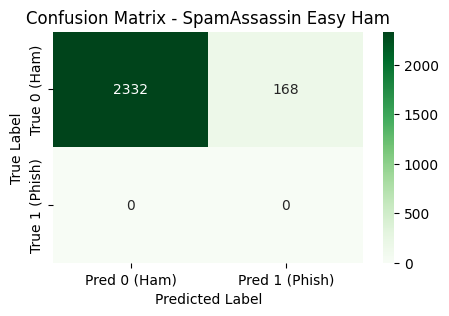
\includegraphics[scale=0.85]{confusion-matrices/random-forest/spamassassin-easy-ham.png}
    \caption{Confusion matrix for Random Forest on SpamAssassin Easy Ham independent test set}
  \end{center}
\end{figure}

\begin{figure}[H]
  \begin{center}
    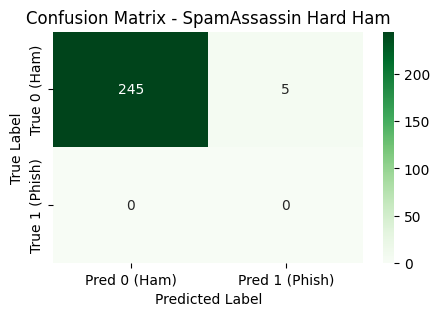
\includegraphics[scale=0.85]{confusion-matrices/random-forest/spamassassin-hard-ham.png}
    \caption{Confusion matrix for Random Forest on SpamAssassin Hard Ham independent test set}
  \end{center}
\end{figure}

\begin{figure}[H]
  \begin{center}
    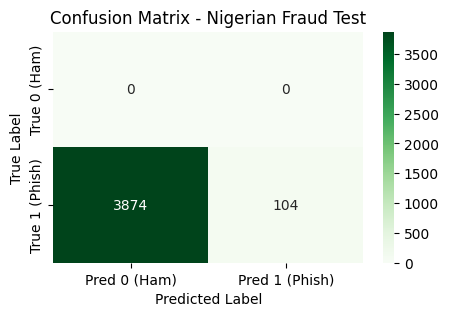
\includegraphics[scale=0.85]{confusion-matrices/random-forest/nigerian-fraud.png}
    \caption{Confusion matrix for Random Forest on Nigerian Fraud independent test set}
  \end{center}
\end{figure}

\begin{figure}[H]
  \begin{center}
    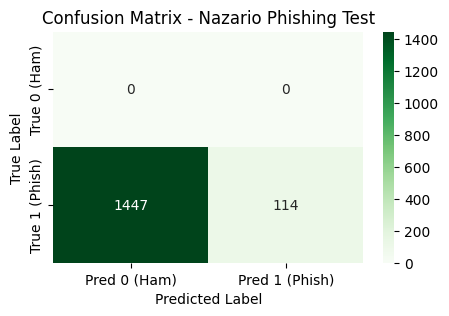
\includegraphics[scale=0.85]{confusion-matrices/random-forest/nazario-spam.png}
    \caption{Confusion matrix for Random Forest on Nazario Phishing independent test set}
  \end{center}
\end{figure}

\begin{figure}[H]
  \begin{center}
    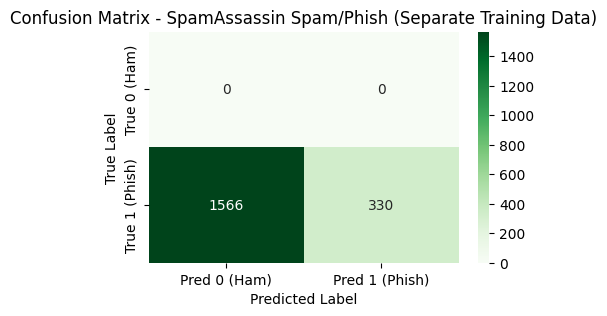
\includegraphics[scale=0.85]{confusion-matrices/random-forest/spamassassin-additional.png}
    \caption{Confusion matrix for Random Forest on an additional SpamAssassin  independent test set}
  \end{center}
\end{figure}

\noindent For the SpamAssassin "Easy Ham" and "Hard Ham" datasets consisting entirely of legitimate emails, i.e. label 0, the model managed to achieve high accuracies of \textbf{0.9328} and \textbf{0.9800} respectively. The precision, recall, and F1-score for the phishing class was 0.0 as expected, as none of these ham emails are phishing -- the model exhibited correct classification behaviour.\newline

\noindent In general, datasets containing solely of either phishing or spam emails, such as Nigerian Fraud, Nazario Phishing, and the additional SpamAssassin dataset, resulted in very low recall scores for the phishing class, i.e. ranging from \textbf{0.0261} to \texttt{0.1741}, disregarding the fact that the model had a perfect precision of \textbf{1.0000} in the instances it did correctly predict an email as phishing. Despite the fact that only a few phishing emails were identified as phishing, it can be seen that the model clearly fails when presented with a vast majority of phishing instances for general data sources (low accuracies and F1-scores). Furthermore, the ROC AUC scores are not applicable (NaN) for these evaluations as the model had a large domination for one particular class.


  % 4.2: XAI for Random Forest using SHAP
  \subsection{XAI for Random Forest using SHAP}
  % ai-phishing-detection-dissertation/report/sections/4-results/xai-for-random-forest-using-shap/gloal-feature-importance.tex

\subsubsection*{Global feature importance}

  % ai-phishing-detection-dissertation/report/sections/4-results/xai-for-random-forest-using-shap/local-explanations-instance-level.tex

\subsubsection*{Local explanations (instance-level)}


  % 4.3: DistilBERT model performance
  \subsection{DistilBERT model performance}
  % ai-phishing-detection-dissertation/report/sections/4-results/random-forest-model-performance/performance-on-internal-test-set.tex

\subsubsection*{Performance on internal test set}

  % ai-phishing-detection-dissertation/report/sections/4-results/random-forest-model-performance/performance-on-independent-test-sets.tex

\subsubsection*{Performance on independent test sets}
The Random Forest model's ability to generalise across different data sources that have unique characteristics was measured against several selected independent datasets. Performance on these datasets are summarised in the below table. Additionally, confusion matrices are presented for each independent set.

\begin{table}[h]
\centering
\begin{tabularx}{\textwidth}{|X|X|X|X|X|X|}
\hline
\textbf{Dataset} & \textbf{Accuracy} & \textbf{Precision (Phish)} & \textbf{Recall (Phish)} & \textbf{F1-Score (Phish)} & \textbf{ROC AUC} \\
\hline
SpamAssassin Easy Ham & \texttt{0.9328} & \texttt{0.0000} & \texttt{0.0000} & \texttt{0.0000} & \texttt{NaN} \\
\hline
SpamAssassin Hard Ham & \texttt{0.9800} & \texttt{0.0000} & \texttt{0.0000} & \texttt{0.0000} & \texttt{NaN} \\
\hline
Nigerian Fraud Test & \texttt{0.0261} & \texttt{1.0000} & \texttt{0.0261} & \texttt{0.0510} & \texttt{NaN} \\
\hline
Nazario Phishing Test & \texttt{0.0730} & \texttt{1.0000} & \texttt{0.0730} & \texttt{0.1361} & \texttt{NaN} \\
\hline
SpamAssassin Spam/Phish (Test Portion) & \texttt{0.1741} & \texttt{1.0000} & \texttt{0.1741} & \texttt{0.2965} & \texttt{NaN} \\
\hline
\end{tabularx}
\caption{Random Forest performance on external test sets}
\end{table}

\begin{figure}[H]
  \begin{center}
    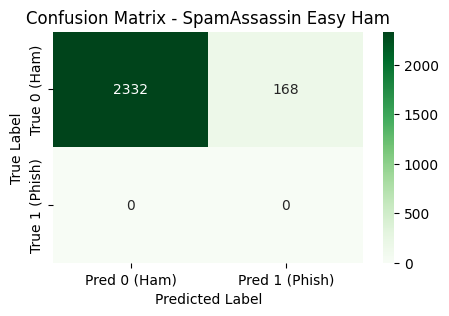
\includegraphics[scale=0.85]{confusion-matrices/random-forest/spamassassin-easy-ham.png}
    \caption{Confusion matrix for Random Forest on SpamAssassin Easy Ham independent test set}
  \end{center}
\end{figure}

\begin{figure}[H]
  \begin{center}
    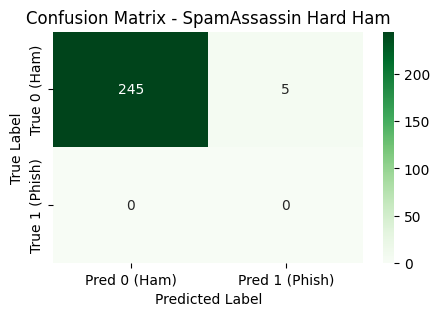
\includegraphics[scale=0.85]{confusion-matrices/random-forest/spamassassin-hard-ham.png}
    \caption{Confusion matrix for Random Forest on SpamAssassin Hard Ham independent test set}
  \end{center}
\end{figure}

\begin{figure}[H]
  \begin{center}
    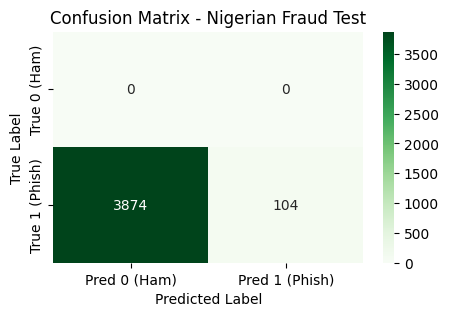
\includegraphics[scale=0.85]{confusion-matrices/random-forest/nigerian-fraud.png}
    \caption{Confusion matrix for Random Forest on Nigerian Fraud independent test set}
  \end{center}
\end{figure}

\begin{figure}[H]
  \begin{center}
    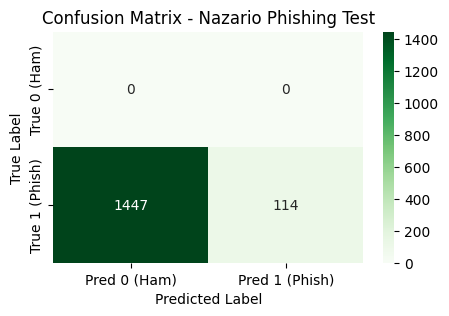
\includegraphics[scale=0.85]{confusion-matrices/random-forest/nazario-spam.png}
    \caption{Confusion matrix for Random Forest on Nazario Phishing independent test set}
  \end{center}
\end{figure}

\begin{figure}[H]
  \begin{center}
    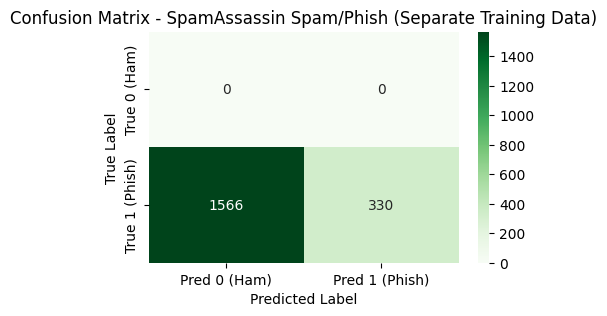
\includegraphics[scale=0.85]{confusion-matrices/random-forest/spamassassin-additional.png}
    \caption{Confusion matrix for Random Forest on an additional SpamAssassin  independent test set}
  \end{center}
\end{figure}

\noindent For the SpamAssassin "Easy Ham" and "Hard Ham" datasets consisting entirely of legitimate emails, i.e. label 0, the model managed to achieve high accuracies of \textbf{0.9328} and \textbf{0.9800} respectively. The precision, recall, and F1-score for the phishing class was 0.0 as expected, as none of these ham emails are phishing -- the model exhibited correct classification behaviour.\newline

\noindent In general, datasets containing solely of either phishing or spam emails, such as Nigerian Fraud, Nazario Phishing, and the additional SpamAssassin dataset, resulted in very low recall scores for the phishing class, i.e. ranging from \textbf{0.0261} to \texttt{0.1741}, disregarding the fact that the model had a perfect precision of \textbf{1.0000} in the instances it did correctly predict an email as phishing. Despite the fact that only a few phishing emails were identified as phishing, it can be seen that the model clearly fails when presented with a vast majority of phishing instances for general data sources (low accuracies and F1-scores). Furthermore, the ROC AUC scores are not applicable (NaN) for these evaluations as the model had a large domination for one particular class.


  % 4.4: XAI for DistilBERT using LIME
  % ai-phishing-detection-dissertation/report/sections/4-results/xai-for-distilbert-using-lime.tex

\subsection{XAI for DistilBERT using LIME}
The following examples below demonstrate the LIME out, highlighting keywords that steered the final decision of the DistilBERT model to the "Phishing" (label 1) class.\newline

\noindent Instance 0: Phishing email with persuasive language

\begin{itemize}
  \item \textbf{Original text snippet}: "\textit{do you have a crying need for bigger and stronger love weapon? we'll tell where to get it! see your tool swell in length and width immensely! the herbert henry dow high school located in midland,he cheered on for alberta's kevin martin. martin won 9 8champions league earlier today after defeating li:won}"
  \item \textbf{Model prediction}: Phishing (predicted class index: 1)
\end{itemize}

\noindent The below figure presents the LIME explanation for Instance 1 for sample email classified as phishing. Here, LIME highlighted terms like "\textit{love}" (approx. weight \textbf{0.056}), "\textit{length}" (approx. weight \textbf{0.051}), "\textit{width}" (approx. weight \textbf{0.037}), "\textit{crying}" (approx. weight \textbf{0.033}), "\textit{stronger}" (approx. weight \textbf{0.033}), and "\textit{bigger}" (approx. weight \textbf{0.028}) as the major influential factors to the classification. It suggests these words are common for deceptive content and aim to invoke an emotional response.

\newpage

\vspace{0.5cm}
\begin{figure}[H]
  \begin{center}
    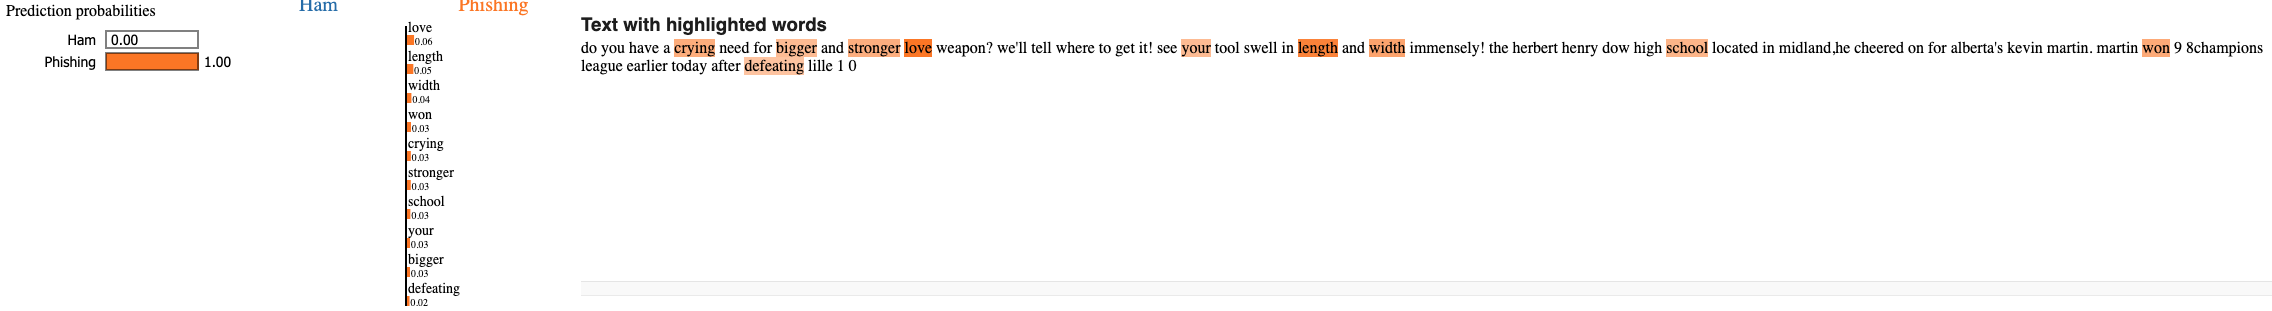
\includegraphics[scale=0.3,angle=90]{xai-visualisations/distilbert/Screenshot 2025-05-26 at 16.11.57.png}
    \caption{DistilBERT LIME explanation for Instance 0}
  \end{center}
\end{figure}

\newpage

\noindent Instance 1: Phishing with potentially misleading content

\begin{itemize}
  \item \textbf{Original text snippet}: "\textit{the daily top 10 from cnn.com top videos and stories as of aug 1, 2008 3 58 pm edt top 10 videos 1. mom parties at a club nancy grace has new photos of casey anthony partying at a nightclub after her daughter caylee vanished. 2. woman's computer spies on her 3. tigers attack teen at zoo 4. mistress}"
  \item \textbf{Model prediction}: Phishing (predicted class index: 1)
\end{itemize}

\noindent Another email that the DistilBERT model classified as phishing, due to terms LIME identified: "\textit{cnn}" (approx. weight \textbf{0.087}), "\textit{videos}" (approx. weight \textbf{0.065}), "\textit{starbucks}" (approx. weight \textbf{0.051}), "\textit{2008}" (approx. weight \textbf{0.046}), and "\textit{top}" (approx. weight \textbf{0.043}). It was surprising that terms like "\textit{trial}" (approx. weight \textbf{0.025}) and "\textit{casey}" (approx. weight \textbf{0.008}) had some slight influence on the classification, but the earlier terms were much stronger.

\newpage

\vspace{0.5cm}
\begin{figure}[H]
  \begin{center}
    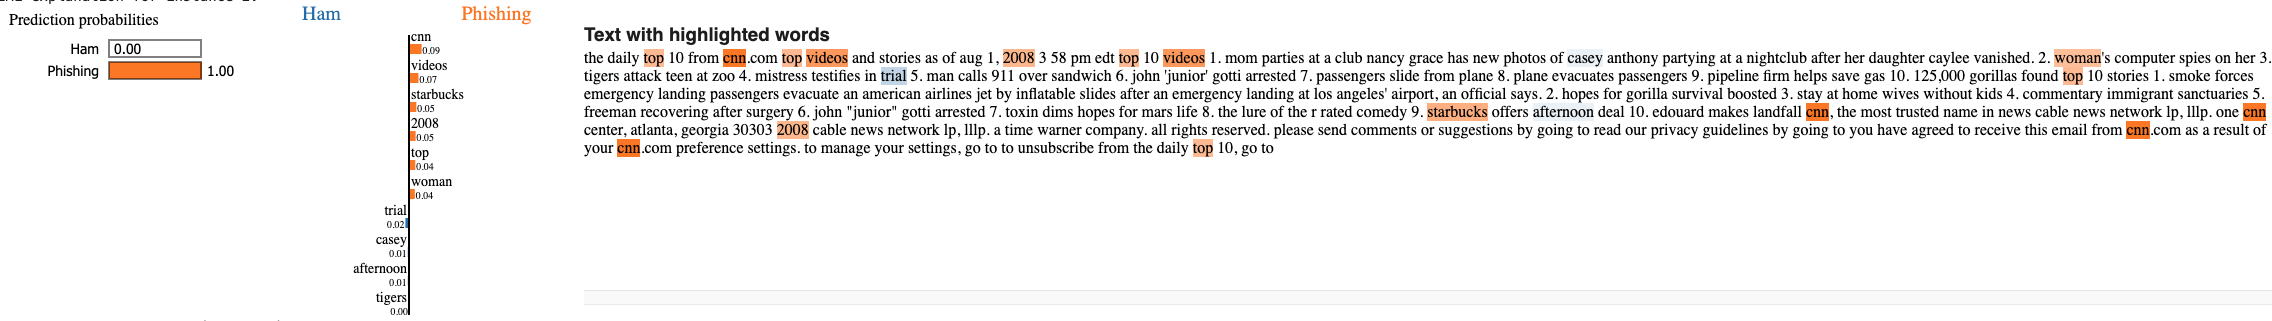
\includegraphics[scale=0.3,angle=90]{xai-visualisations/distilbert/Screenshot 2025-05-26 at 16.12.34.png}
    \caption{DistilBERT LIME explanation for Instance 1}
  \end{center}
\end{figure}

\newpage

\noindent Instance 2: Phishing email with urgent/action-oriented phrasing

\begin{itemize}
  \item \textbf{Original text snippet}: "\textit{approved, medicine fast delivery check out here}"
  \item \textbf{Model prediction}: Phishing (predicted class index: 1)
\end{itemize}

\noindent The final email instance was also classified as phishing, and the LIME explanation below demonstrates how terms such as "\textit{medicine}" (approx. weight \textbf{0.514}), "\textit{delivery}" (approx. weight \textbf{0.239})m and "\textit{fast}" (approx. weight \textbf{0.229}) all contribute strongly to the phishing classification. Terms like "\textit{approved}" did not have much of a significant impact. This shows the sensitive nature of the model to specific keywords.

\newpage

\vspace{0.5cm}
\begin{figure}[H]
  \begin{center}
    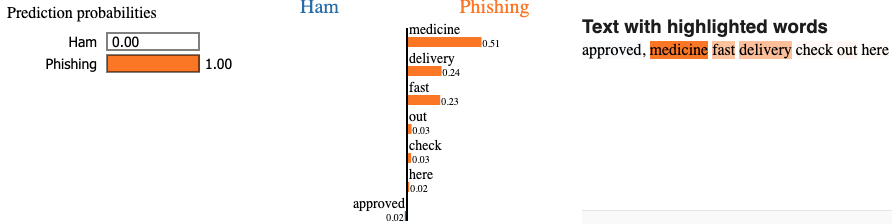
\includegraphics[scale=0.75,angle=90]{xai-visualisations/distilbert/Screenshot 2025-05-26 at 16.14.19.png}
    \caption{DistilBERT LIME explanation for Instance 2}
  \end{center}
\end{figure}


  % 4.5: Comparative performance summary
  % ai-phishing-detection-dissertation/report/sections/4-results/conparative-performance-summary.tex

\subsection{Comparative performance summary}
A direct comparison between both the Random Forest and DistilBERT model will be presented and summarised. The main aim of this comparison is to focus on how the performance on the internal test set from the combined training corpus as well as their generalisation ability on independent data sources. The below table provides a side-by-side comparison of these metrics, with specific attention weighted F1-scores and accuracies.

\begin{table}[h]
\centering
\begin{tabularx}{\textwidth}{|X|X|X|}
\hline
\textbf{Metric / Dataset} & \textbf{Random Forest} & \textbf{DistilBERT} \\
\hline
\textbf{Internal Test Set (Enron+CEAS Split)} & & \\
\hline
Accuracy & \texttt{0.9815} & \texttt{0.9973} \\
F1-Score (Phishing, Label 1) & \texttt{0.9824} & \texttt{0.9974} \\
ROC AUC & \texttt{0.9988} & \texttt{1.0000} \\
\hline
\textbf{Independent Test Set: Nazario Phishing} & & \\
\hline
Accuracy & \texttt{0.0730} & \texttt{0.3773} \\
F1-Score (Phishing, Label 1) & \texttt{0.1361} & \texttt{0.5479} \\
Recall (Phishing, Label 1) & \texttt{0.0730} & \texttt{0.3773} \\
\hline
\textbf{Independent Test Set: Nigerian Fraud} & & \\
\hline
Accuracy & \texttt{0.0261} & \texttt{0.3175} \\
F1-Score (Phishing, Label 1) & \texttt{0.0510} & \texttt{0.4820} \\
Recall (Phishing, Label 1) & \texttt{0.0261} & \texttt{0.3175} \\
\hline
\textbf{Independent Test Set: SpamAssassin Spam/Phish} & & \\
\hline
Accuracy & \texttt{0.1741} & \texttt{0.2827} \\
F1-Score (Phishing, Label 1) & \texttt{0.2965} & \texttt{0.4408} \\
Recall (Phishing, Label 1) & \texttt{0.1741} & \texttt{0.2827} \\
\hline
\end{tabularx}
\caption{Comparison of Random Forest and DistilBERT on the internal and external datasets}
\end{table}

\noindent There is an exceptionally high performance observed on the internal test set, with DistilBERT achieving near perfect scores on all metrics outperforming Random Forest. However when evaluated on independent test sets consisting of either entirely phishing or spam emails. Both models did not perform well in their overall accuracy and F1-scores here for phishing classes, although precision was high with low recall. But on the more challenging external datasets, DistilBERT achieved higher weighted F1-scores and recall values than Random Forest, performing relatively better -- whilst still limited. Both models missed out on a large proportion of actual phishing emails to be marked as "spam".


  % 4.6: User feedback on XAI explanations
  % ai-phishing-detection-dissertation/report/sections/4-results/user-feedback-for-xai-explanations.tex

\subsection{User feedback on XAI explanations}
To gather some preliminary insights into the generated explanations and assess their user-friendly aspects, a small group of peers were selected to solicit informal, qualitative feedback from them. Each of the peers (around 4 or 5 selected), were first shown the Random Forest SHAP waterfall plot, as well as a DistilBERT LIME explanation, along with the corresponding email instance and relevant model classification outcome.\newline

\noindent General, open-ended questions were asked on the effectiveness and clarity of the explanations, and how they highlighted the features in which the model was largely influenced by. Their perceived trustworthiness of each particular model was noted. Questions included, but were not limited to:

\begin{enumerate}
  \item "\textit{How clear is this generated explanation to you, in aiding your understanding for the model's prediction?}"
  \item "\textit{Do the generated explanations increase your trust in AI-based systems (if any beforehand)?}"
  \item "\textit{What aspects of this generated explanation are specifically helpful to you?}"
  \item "\textit{Do you prefer the SHAP waterfall plots of the LIME word-level highlighting?}"
\end{enumerate}

\noindent The responses were varies and ranged, indicating several themes of both trust coupled with confusion. Participants were found to generally prefer the word-level highlighting of DistilBERT's LIME explanations to be more helpful, than the SHAP waterfall plot. A few of the participants took a liking to the vertical, visually colour-coded waterfall plots with arrows to indicate what features skewed the prediction. An individual noted that they would have liked to seen a combination of both waterfall plots and word-level highlighting for both models, for a more helpful. The responses amongst this were split evenly, with no clear, overwhelming bias for either.\newline

\noindent It's important to note that the generated explanations definitely increased understanding, and raised the baseline levels of default trust a typical user would instil in the system. Some users still had doubt in the system regardless however, reserving their skepticism on the AI systems regardless of understanding their decision-making processes. Some participants revealed that the XAI explanations did not whatsoever impact their trust on the models, and their interaction with the system would remain the same. One participant raised a point that the explanations could perhaps be misleading if the model was focusing on the wrong terms or features. Another mentioned how their trust would solely be based upon the numerical, performance metrics of the model such as accuracy, prevision, recall, and F1-score.\newline

\noindent These observations, whilst informal and limited in sample size, still form an initial basis to further optimise user-centric XAI applications.


  \newpage

  % 5: Discussion
  \section{Discussion}\label{sec:5-discussion}
  % ai-phishing-detection-dissertation/report/sections/3-research-methodology/model-development/introduction.tex



  % 5.1: Interpretation of model performance
  \subsection{Interpretation of model performance}
  % ai-phishing-detection-dissertation/report/sections/4-results/random-forest-model-performance/performance-on-internal-test-set.tex

\subsubsection*{Performance on internal test set}

  % ai-phishing-detection-dissertation/report/section/5-discussion/interpretation-of-model-performance/generalisation-challenges-on-independent-test-sets.tex

\subsubsection*{Generalisation challenge on independent test sets}
There was a very contrasting observation in the performance for both models, when evaluated on a selection of external, independent test sets. While both models achieved excellent scores on the internal test set of the Enron-CEAS distribution, the models fall short for general phishing and legitimate emails.\newline

\noindent A consistent trend was seen for both models on these external datasets:

\begin{itemize}
  \item \textbf{Precision for the phishing class remained high, often at 1.0000}. The models recognised emails as phishing from these data sources, and often got them correct.
  \item Likewise, \textbf{precision for the ham class remained high, often at 1.0000}. The models recognised emails as legitimate from these data sources, and got almost all instances correct.
  \item \textbf{The recall for the phishing class was very low, from approx. 0.02 to 0.38}. Both models missed many of the actual phishing emails in these sources, and were actually classed as legitimate.
  \item A low recall impacts the \textbf{overall accuracy and F1-scores} of these models, resulting in very low scores.
\end{itemize}


  % 5.2: Insights from XAI
  \subsection{Insights from XAI}
  % ai-phishing-detection-dissertation/report/section/5-discussion/xai-insights/random-forest-shap-explanations.tex

\subsubsection*{Random Forest (SHAP) explanations}
SHAP being applied to the Random Forest model presented the following insights:

\begin{itemize}
  \item \textbf{Global feature importance}: The SHAP summary plot highlighted the TF-IDF features that had the most influence on the model's final classification. For example, terms such as "\textit{enron}", "\textit{email}", "\textit{2008}", "\textit{subject}", and "\textit{thanks}", showing a global significance. The plot was vital in visually representing how the presence of terms with high Shapley values either pushed classifications to phishing (positive) or legitimate (negative). A global view was helpful in knowing what general patterns the Random Forest model came to realise for each class.
  \item \textbf{Local instance explanations}: SHAP waterfall plots on the other hand were localised for each individual email instance prediction:
  \begin{itemize}
    \item For email instances correctly predicted as legitimate, the SHAP values show that terms like "\textit{attached}", "\textit{forwarded}", and "\textit{review}" (for Instance 1) contribute the most to this. Professional communication language generally means a lower probability of phishing. This is valid since legitimate emails usually consist of professional language.
    \item For email instances correctly predicted as phishing, the explanations show that some terms like "\textit{sex}", "\textit{things}", as well as nonsensical terms like "fa", "ed", and "es" (for Instances 2 and 3) as key indicators in the model marking an email as phishing. Here however, there is no consistent pattern observed consistent with typical phishing emails, but the presence unusual characters is typical spam content.
    \item The local explanations generated show that the model had a dependency on certain textual components within the TF-IDF features, on which it performed well for on the internal test set. But it was difficult (and more detail was required) on understanding how these TF-IDF features themselves has a contribution to the overall classifications, specifically relating to their technical details (i.e. terms or n-grams) rather than just in a semantic context.
  \end{itemize}
\end{itemize}

  % ai-phishing-detection-dissertation/report/section/5-discussion/xai-insights/distilbert-lime-explanations.tex

\subsubsection*{DistilBERT (LIME) explanations}
Explanations for the fine-tuned DistilBERT model were generated with LIME. The following was revealed:

\begin{itemize}
  \item \textbf{DistilBERT (LIME) explanations}: The LIME visualisations show how each specific word within an email instance most contributed to the final prediction.
  \begin{itemize}
    \item LIME identified words like "\textit{love}", "\textit{length}", "\textit{width}", "\textit{crying}", and "\textit{stronger}" (from Instance 0) as contributions to the phishing decisions the model makes. Spam emails usually try and invoke a response from a user as part of their tactics, and words like so are often used to achieve this.
    \item Additionally, terms like "\textit{cnn}", "\textit{videos}", and "\textit{starbucks}" were highlighted by the LIME explanation (from Instance 1), marking these words as phishing. This is once again consistent with spam email tactics, who often use fake news updates to trick users with. Furthermore, LIME also showed some other words like "\textit{trial}" and "\textit{casey}" that push a classification away from the phishing label. The model is capable of catching conflicting signals.
    \item LIME explanations also strongly weights terms like "\textit{medicine}", "\textit{delivery}", and "\textit{fast}" (from Instance 2), even if the email instance is concise and short. It matches common keywords used in spam emails.
  \end{itemize}
  \item \textbf{Interpretability of LIME}: The word-level highlighting of LIME makes these explanations more easier to understand and comprehend than SHAP initially. Specific text components, that led to the final decision, can be singled out and analysed separately. This helps to provide a more direct semantic relation, rather than explaining the TF-IDF features via SHAP for the Random Forest model
\end{itemize}

  % ai-phishing-detection-dissertation/report/section/5-discussion/xai-insights/comparing-and-reflecting-on-xai-techniques-and-model-behaviour.tex

\subsubsection*{Comparing and reflecting on XAI techniques and model behaviour}
From analysing the XAI explanations, it can be said that:

\begin{itemize}
  \item The Random Forest model, using SHAP, shows a clear view of which specific TF-IDF features contributed most to individual email instances. This is critical for understanding the model on a feature engineering level.
  \item With DistilBERT, using LIME, it provided a more semantic understanding of its local explanations, by directly acknowledging the specific words. This is more helpful for users to understand why and what parts of text was predicted to the relevant class.
\end{itemize}

\noindent When it comes to the generalisation challenges observed earlier, both models performed poorly on all the external, independent test sets. Now whilst XAI was applied mainly to email instances on the internal test set, applying the same techniques to instances across the external data sources would potentially give insight into the decision making processes that led to incorrect results. This would reveal the following:

\begin{itemize}
  \item Patterns that the models were trained on, from the training distribution, aren't present in the external emails.
  \item For Random Forest, the key vocabulary from the "\textit{TfidfVectorizer}" was lacking in external phishing emails.
  \item For DistilBERT, the fine-tuning process was conducted on the training distribution, making it possibly quite sensitive to language structures and semantics attributed to the Enron/CEAS training set.
\end{itemize}


  % 5.3: Answering research questions and objectives
  \subsection{Answering research questions and objectives}
  % ai-phishing-detection-dissertation/report/section/5-discussion/answering-research-questions-and-objectives/primary-research-question.tex

\subsubsection*{Primary research question}
"\textit{How can Explainable AI (XAI) improve the usability and trustworthiness of AI-based phishing detection systems without compromising on accuracy?}"

\begin{itemize}
  \item \textbf{Accuracy}: From this study, the Random Forest and DistilBERT models achieved very high accuracies, 0.9815 and 0.9973 respectively, on the internal test set comprised of Enron ham and CEAS 2008 phishing emails. XAI techniques, SHAP for Random Forest and LIME for DistilBERT, were applied as an analysis to the model's decision making process, and did not in any way affect the predictive accuracy when tested on the internal set. So for in-distribution data, it's safe to conclude that XAI doesn't have any affect on the accuracy. However, the generalisation limitations on external, independent datasets show that accuracy on in-distribution data cannot apply, and guarantee a similar or reasonable performance, on different distributions of data. This is an area that XAI can help demystify.
  \item \textbf{Usability and trustworthiness}:
  \begin{itemize}
    \item Analysing the generated SHAP and LIME explanations qualitatively did indeed acknowledge that XAI gives insight into the behaviour and decision making processes of a model. The word-based highlighting by LIME proved to be more superior in its understandability, but this is not to disregard the difference in perspective that SHAP provides for Random Forest, in terms of exploring the significant of TF-IDF terms on the model's overall classification.
    \item Preliminary, informal user feedback was solicited from a small group of participants. The feedback gives pointers to enhancing explanations for both models, especially for Random Forest. There were varying responses on the trust, clarity of explanations, and overall usefulness of the generated explanations, coupled with pre-existing notions participants had about AI.
  \end{itemize}
\end{itemize}

  % ai-phishing-detection-dissertation/report/section/5-discussion/answering-research-questions-and-objectives/sub-research-questions.tex

\subsubsection*{Sub research questions}

\begin{enumerate}
  \item \uline{\textbf{SUB RESEARCH QUESTION 1}}: "\textit{What are the current limitations of AI phishing detection models in terms of their usability and interpretability?}"
  \begin{itemize}
    \item \hyperref[sec:2-literature-review]{\uline{\textbf{Section 2}}} conducts a comprehnsive literature review on that covers the current state of AI models in the context of phishing detection and how most of them are inherently "black-boxed". It also explores how although transformer models, like DistilBERT for example, can achieve a high accuracy for classification tasks like phishing detection, their inner workings are obscured and hard to understand. This underscores the need for XAI techniques such as SHAP and LIME to allow these models to become more interpretable and be trustworthy enough to be deployed in a wide range of settings. The practical limitations when implementing this study are detailed in \hyperref[sec:5-discussion]{\uline{\textbf{Section 5}}}.
  \end{itemize}
  \item \uline{\textbf{SUB RESEARCH QUESTION 2}}: "\textit{How do the interpretability features affect a user's trust building and decision-making processes?}"
  \begin{itemize}
    \item The informal user feedback collected addresses this research question. Responses varied, but most were positively accepting of the XAI explanations as a way to increase their trust in an AI system, as well as being able to somewhat understand the inner workings behind the decision making and classificaion processes through the visualisations. All observations are detailed \hyperref[sec:4-results]{\uline{\textbf{Section 4}}}.
  \end{itemize}
  \item \uline{\textbf{SUB RESEARCH QUESTION 3}}: "\textit{How can XAI techniques, i.e. SHAP and LIME, be integrated efficiently on top of existing AI phishing detection models?}"
  \begin{itemize}
    \item The study took two basline models, Random Forest (via sckit-learn) and DistilBERT (via Hugging Face), and integrated SHAP with TF-IDF features and LIME respectively. The implementation is covered in \hyperref[sec:3-research-methodology]{\uline{\textbf{Section 3}}}, showing the entire process from preprocessing to evaluation to XAI explanation generation. In terms of efficiency, this concerns the computational costs for training both models, concerning the training times and generation of XAI explanations (individual email instances demonstrated in \hyperref[sec:4-results]{\uline{\textbf{Section 4}}}).
  \end{itemize}
\item \uline{\textbf{SUB RESEARCH QUESTION 4}}: "\textit{What trade-offs, if any, arise between the performance and interpretability of the AI phishing detection model?}"
  \begin{itemize}
    \item For this study, XAI techniques were applied after the models were trained. The application of these techniques did not in anyway impact the performance of either the Random Forest or the DistilBERT models. There were no trade-offs concerning the accuracy per say, but there was in the complexity of the model against the type of explaination that can be generated. For example, direct feature importance from Random Forest via SHAP on the TDF-IDF features, compared to the word-level highlighting for DistilBERT via LIME. Another major trade-off is the model's exceptional performance on internal data compared to general data -- XAI can be implemented here to address this.
  \end{itemize}
\end{enumerate}

  % ai-phishing-detection-dissertation/report/section/5-discussion/answering-research-questions-and-objectives/achievement-of-project-objectives.tex

\subsubsection*{Achievement of project objectives}



  \newpage

  % 6: Conclusion
  \section{Conclusion}\label{sec:6-conclusion}

  \newpage

  % 7: References
  \bibliographystyle{agsm}
  \addcontentsline{toc}{section}{References}
  \bibliography{bibliography}

  \newpage

  % 8: Appendices
  \section*{Appendices}
\addcontentsline{toc}{section}{Appendices}

\subsection*{Appendix 1: Ethical approval form}
\addcontentsline{toc}{subsection}{Appendix 1: Ethical approval form}
\label{sec:Appendix 1}

\includepdf[pages=-,scale=0.75]{images/ethical-approval-form.pdf}

\newpage

\subsection*{Appendix 2: Ethical courses certificates}
\addcontentsline{toc}{subsection}{Appendix 2: Ethical courses certificates}
\label{sec:Appendix 2}

\begin{figure}[htbp]
    \centering
    
\includegraphics[width=0.5\textwidth]{images/ethics-in-research-badge.png}
    \caption{Ethics in research badge}
\end{figure}

\begin{figure}[htbp]
    \centering
    
\includegraphics[width=0.5\textwidth]{images/ethical-approval-process-badge.png}
    \caption{Ethical approval badge}
\end{figure}

\begin{figure}[htbp]
    \centering
    \includegraphics[width=1\textwidth]{images/epigeum-certificate.png}
    \caption{Epigeum certificate}
\end{figure}

\begin{figure}[htbp]
    \centering
    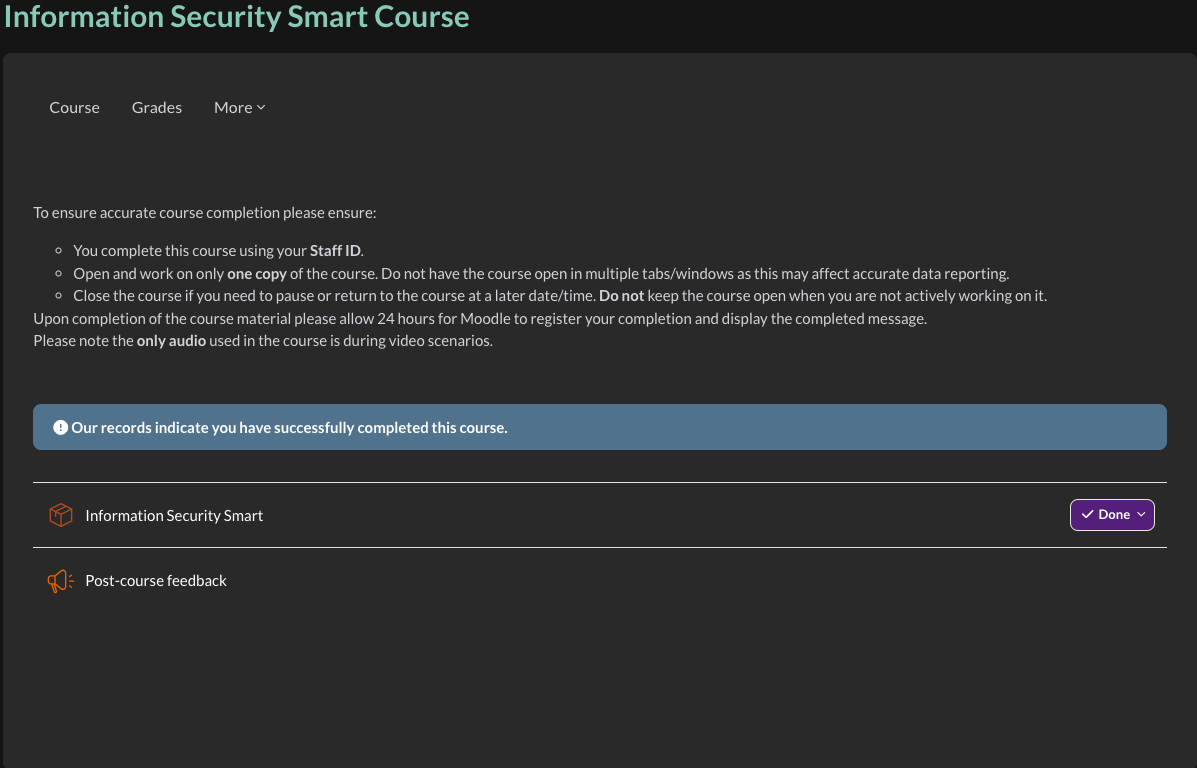
\includegraphics[width=1\textwidth]{images/information-security-smart-certificate.png}
    \caption{Information SMART certificate}
\end{figure}

\newpage

\subsection*{Appendix 3: Project plan}
\addcontentsline{toc}{subsection}{Appendix 3: Project plan}
\label{sec:Appendix 3}

\begin{longtable}{|p{5cm}|p{6cm}|p{4cm}|}
    \hline
    \textbf{Phase} & \textbf{Tasks} & \textbf{Duration} \\
    \hline
    \endfirsthead
    \hline
    \textbf{Phase} & \textbf{Tasks} & \textbf{Duration} \\
    \hline
    \endhead
    
    \hline
    \endfoot
    
    \hline
    \endlastfoot
    
    Research and Planning & 
    \begin{itemize}
        \item Conduct literature review.
        \item Refine research questions and objectives.
        \item Identify datasets (e.g., PhishTank, Kaggle).
    \end{itemize} & 
    End Jan – Early Feb (1–2 weeks) \\
    \hline
    
    Dataset Preparation & 
    \begin{itemize}
        \item Clean and preprocess data.
        \item Perform feature extraction (e.g., URLs, metadata).
        \item Split data into training, validation, and test sets.
    \end{itemize} & 
    Early Feb (1–2 weeks) \\
    \hline
    
    Model Development & 
    \begin{itemize}
        \item Develop baseline model (e.g., Random Forest, Logistic Regression).
        \item Experiment with advanced models (e.g., BERT).
        \item Train and validate models.
    \end{itemize} & 
    Mid-Feb – Early Mar (3 weeks) \\
    \hline
    
    Integration of XAI & 
    \begin{itemize}
        \item Implement SHAP and LIME for interpretability.
        \item Visualize explanations (e.g., feature importance, email components).
        \item Ensure explanation clarity and usability.
    \end{itemize} & 
    Early Mar – Mid-Mar (2 weeks) \\
    \hline
    
    Evaluation and Comparison & 
    \begin{itemize}
        \item Evaluate model performance (accuracy, F1-score).
        \item Assess interpretability using metrics (faithfulness, stability).
        \item Compare XAI-enhanced system to black-box models.
    \end{itemize} & 
    Mid-Mar – End Mar (2 weeks) \\
    \hline
    
    Report Writing & 
    \begin{itemize}
        \item Write methodology, results, and discussion sections.
        \item Proofread and finalize dissertation.
        \item Integrate appendices (e.g., Gantt chart, ethical approval).
    \end{itemize} & 
    April – Mid-May (5–6 weeks) \\
    \hline
    
    \end{longtable}
    


\end{document}
